\documentclass[a4paper, 10pt, headings=standardclasses, oneside, bibliography=totocnumbered]{scrbook}

\usepackage{stylesheet}

\title{Thoughts About Writing~\hologo{LaTeX}}
\subtitle{Some \hologo{LaTeX} Do’s and Don’ts}
\author{Jendrik Stelzner}
\date{\today}
\publishers{
  Available at \texttt{\url{https://github.com/cionx/thoughts-about-writing-latex}.}
  \\
  Please send comments and corrections to \texttt{\href{mailto:stelzner@uni-bonn.de}{stelzner@uni-bonn.de}.}
}
  
\begin{document}

\frontmatter

\maketitle
\setchapterpreamble{
  \dictum[German saying]{Das Auge liest mit.}
  \vspace{1em}
}

\chapter{Preface}

This text presents some thoughts about what (not) to do in mathematical typesetting using \hologo{LaTeX}.
Examples are provdided using the \texttt{tcolorbox} package.
This text is not intended as a first introduction to \hologo{LaTeX}.
Some of the following remarks are subject to individual taste.

\tableofcontents


\mainmatter
\chapter{Before you start writing}

A dozen mistakes and bad choices can be made before even the first word of actual text is written.
In this chapter we talk about how to prevent this from happening.
Some of the points -- those about code quality and code management -- are not unique to writing {\LaTeX}.




\section{Use version control}

Use some kind of sensible version control\index{version control} for your code.
The author uses Git\index{Git} but has also heard good things about Mercurial\index{Mercurial}.
Sending code to yourself on Facebook\index{Facebook} is not a proper system of version control.





\section{Code quality}



\subsection{Make use of whitespace to organize the code}

The {\LaTeX} compiler almost never cares about unnecessary whitespace in your code.
Use generous amounts of whitespace to organize your code in a sensible way.
Don’t do the following:
\begin{showcode}{Code is too cramped}
\[\begin{pmatrix*}[r]a^2+b^2&a^2-b^2\\-a^2+b^2&-a^2-b^2\end{pmatrix*}\]
\end{showcode}
Instead do the following:
\begin{showcode}{Code is less cramped}
\[
  \begin{pmatrix*}[r]
     a^2 + b^2 &  a^2 - b^2 \\
    -a^2 + b^2 & -a^2 - b^2
  \end{pmatrix*}
\]
\end{showcode}
You can (and should) even do the following:
\begin{showcode}{Code isn’t cramped}
\[
  \begin{pmatrix*}[r]
    a^2 + b^2
    &
    a^2 - b^2
    \\
    - a^2 + b^2
    &
    - a^2 - b^2
  \end{pmatrix*}
\]
\end{showcode}
This last one is easiest to write and easiest to navigate.

Also put at least one space between any two symbols that do not belong together.
Don’t do the following:
\begin{showcode}{Unrelated symbols need to be separated}
$y=\sin(x)-e^x$
\end{showcode}
Instead do the following:
\begin{showcode}{Unrelated symbols are separated}
$y = \sin(x) - e^x$
\end{showcode}
One could (and probably should) go even further and do the following:
\begin{showcode}{Unrelated symbols are separated even better}
$y = \sin ( x ) - e^x$
\end{showcode}



\subsection{Write one sentence per line}

Related the previous point, write at most one sentence per line.
This has at least three advantages:
\begin{itemize}
  \item
    When an error\index{error} or warning\index{warning} occurs {\LaTeX} will (try to) tell you the line of source code in which the problem occurs.
    Having your source code split up over multiple lines makes it much easier to find the problem.
  \item
    Organizing the source code in lines will in most cases make the tools provided by your version control\index{version control} system more efficient to use.
  \item
    By writing one sentence per line you will more easily spot sentences which are overly long.
\end{itemize}



\subsection{Properly indent your source code}

Writing {\LaTeX} means writing source code.
Make sure that your source code is properly indented\index{indentation}.



\subsection{Use \inlinecodetitle{\%} for problematic line~breaks}

Sometimes a sensible line break in your source code can lead to unwanted effects in the resulting output.
Consider the following example:
\begin{showlatex}*{Wrong spacing before a footnote}
Here is some text.
\footnote{Here is a footnote for this text.}
\end{showlatex}
Note the unwanted space\index{before a footnote} between the period and the superscript of the footnote\index{footnote}.
This unwanted space comes from the line break that occurs between them in the source code.
By ending the first line with \inlinecode{\%}\massindex{\%}[\inlinecode] we can \enquote{comment out} this line break.
We hence do the following:
\begin{showlatex}*{Right spacing before a footnote}
Here is some text.%
\footnote{Here is a footnote for this text.}
\end{showlatex}





\section{The compilation process}



\subsection{Use \texorpdfstring{\LuaLaTeX}{LuaLaTeX} or \texorpdfstring{\XeLaTeX}{XeLaTeX}}

Use {\LuaLaTeX}\index{LuaLaTeX@{\LuaLaTeX}} or {\XeLaTeX}\index{XeLaTeX@{\XeLaTeX}} for native Unicode\index{Unicode} support (i.e.\ without including any kind of additional packages).
The author recommends {\LuaLaTeX} because the \packname{microtype}\massindex{microtype}[\packname] package his only a limited functionality under {\XeLaTeX}.



\subsection{Don’t ignore warnings}

There are two ways in which {\LaTeX} will tell you that something went wrong:
Errors\index{error} and warnings\index{warning}.

The occurrence of an error means that {\LaTeX} was unable the process the source code and gave up at some point in the process.
In the case of a warning {\LaTeX} again wasn’t able to process the source code, but decided to produce some output nevertheless.
Hence the only difference between an error and a warning is how {\LaTeX} decided to proceed with it.
But there is no intrinsic difference between the two of them.

It is typically hard to ignore errors, as no output file will be generated.
But warnings also shouldn’t be ignored:
While the occurrence of an error means that you get no output at all, the occurrence of a warning means that you’re getting a faulty output.

% TODO: Too many warnings make future problems worse.





\section{Splitting up a project into multiple files}
\index{including files!zzzz@\igobble |see{file inclusion}}

Any slightly larger project should be split up into multiple files.



\subsection{The commands~\comtitle{usepackage}, \comtitle{include}, \comtitle{input}}

There are (at least) three useful ways to include another file into your project: \comname{usepackage}\massindex[file inclusion]{usepackage}[\comname], \comname{include}\massindex[file inclusion]{include}[\comname] and \comname{input}\massindex[file inclusion]{input}[\comname].
\begin{itemize}[leftmargin=*]
  \item
    Most of the preamble information -- including of packages, configuration of styles, configuration of the look and feels of the document -- should be put into one or multiple \filename{sty}-files.
    These file(s) can then be included into the document by using \comname{usepackage}\massindex[file inclusion]{usepackage}[\comname].
  \item
    The commands~\comname{include} and~\comname{input} insert the text of the specified documents at the position where they are used, but have slight differences:
    \begin{itemize}[label = \textopenbullet, leftmargin=*]
      \item
        The command~\comname{include}\massindex[file inclusion]{include}[\comname] ensures that the specified content starts on a new page, and also that the following content begins on a new page.
        The command~\comname{input}\massindex[file inclusion]{input}[\comname] simply inserts the specified content at the given position without any such additional formatting.
      \item
        The command~\comname{include} cannot be nested:
        The specified file is not allowed to include the command~\comname{include} again.
    \end{itemize}
\end{itemize}

One should use the command~\comname{include} for chapters and the command~\comname{input} for any smaller level of text organization.
One should in particular break the main text into smaller units until each of them can be put into its own file of sensible length.

Suppose for example that your text consists of three chapters, each of which consists of two sections.
Then you should have at least ten files:
\begin{itemize}
  \item
    A master file \filename{main.tex}.
    This file includes all other files in some way, and this is the file which needs to be compiled.
  \item
    A file \filename{mystyle.sty} in which packages are included and options are set.
  \item
    Three files like \filename{chapter1.tex}, \filename{chapter2.tex} and \filename{chapter3.tex} for the chapters.
  \item
    Six files for the sections, say \filename{section1.tex} up to \filename{section6.tex}.
\end{itemize}
These files should include each other as shown in \cref{file inclusion structure}.
\begin{figure}[tb]
  \begin{center}
    % the following diagram uses the "trees" library
    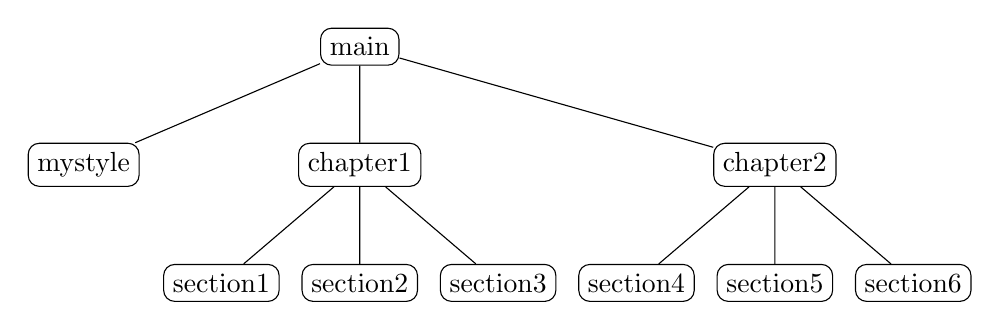
\begin{tikzpicture}[
      every node/.style = {shape=rectangle, rounded corners, draw, align=center},
      level 1/.style = {sibling distance = 15em},
      level 2/.style = {sibling distance = 5em}
      ]
      \node {\filename{main}}
        child { node [right=3em] {\filename{mystyle}} }
        child { node {\filename{chapter1}}
          child { node {\filename{section1}} }
          child { node {\filename{section2}} }
          child { node {\filename{section3}} }
        }
        child { node {\filename{chapter2}}
          child { node {\filename{section4}} }
          child { node {\filename{section5}} }
          child { node {\filename{section6}} }
        };
    \end{tikzpicture}
  \end{center}
  \caption{Splitting up a project into files.}
  \label{file inclusion structure}
\end{figure}
We suppose for simplicity that all ten files are contained in the same directory.
The master file \filename{main.tex} should look roughly as follows:
%
\begin{showcode}{Layout of \filename{main.tex}}
\documentclass[a4paper, 10pt]{scrreprt}

\usepackage{mystyle}

\title{A Report}
\author{John Doe}

\begin{document}

\maketitle

\include{chapter1}
\include{chapter2}

\end{document}
\end{showcode}
%
The file \filename{mystyle.sty} may look as follows:
%
\begin{showcode}{Layout of \filename{mystyle.sty}}
%%%%% PACKAGES

% general mathematics
\usepackage{mathtools}
\usepackage{amssymb}

% commutative diagrams
\usepackage{tikz-cd}

%%%%% NEW COMMANDS

% new operators
\DeclareMathOperator{\End}{End}
\DeclareMathOperator{\Hom}{Hom}
\end{showcode}
%
The file \filename{chapter1.tex} should look roughly as follows:
%
\begin{showcode}{Layout of \filename{chapter1.tex}}
\chapter{Name of the first chapter}

Some introduction to this chapter before the first section appears.

\input{section1}
\input{section2}
\end{showcode}
%
The file \filename{section1.tex} should look roughly as follows:
%
\begin{showcode}{Layout of \filename{section1.tex}}
\section{Name of the first section}

Text of the first section.
\end{showcode}



\subsection{Use \comtitle{includeonly}}

As a document grows so does the time that is needed to compile it.
It is therefore often desirable to compile only certain parts of the document.
One naive solution to this problem is to simply not include the currently unwanted parts, e.g.\ by commenting out the corresponding lines of~\comname{include} and~\comname{input}.
This approach has the problem that references to the now-excluded parts of the document will not compile properly.
This problem can be fixed by using the command~\comname{inludeonly}\massindex[file inclusion]{includeonly}[\comname].

Suppose that your main document, say \filename{main.tex}, included two other files, say \filename{chapter1.tex} and \filename{chapter2.tex}, via the command \comname{include}.
Hence the file~\filename{main.tex} should look roughly as follows:
\begin{showcode}{Basic example of \filename{main.tex}}
\documentclass[a4paper, 10pt]{scrreprt}

\begin{document}

\include{chapter1}
\include{chapter2}

\end{document}
\end{showcode}
By putting~\inlinecode{{\tbs}includeonly\{chapter1\}} in the preamble we tell {\LaTeX} to only compile this specific chapter.
\begin{showcode}{Using the command~\comname{includeonly}}
\documentclass[a4paper, 10pt]{scrreprt}

\includeonly{chapter1}
\begin{document}

\include{chapter1}
\include{chapter2}

\end{document}
\end{showcode}
If in the above situation chapter~1 contains some references to chapter~2 then these references will still compile correctly, even though only chapter~1 is compiled.

The command~\comname{includeonly} has two quirks, which follow from the way {\LaTeX} handles referencing:

When {\LaTeX} compiles the file~\filename{main.tex} an auxiliary file~\filename{main.aux} is created.
This file contains various information about the compiled document.
It does in particular contain a list of all labels found in \filename{main.tex} during the compilation process.
The next compilation process can then access these information to properly properly typeset all references that refer to these labels.

A feature of the command~\comname{include} (which the command~\comname{input} does not have) is that such an auxiliary file is also generated for the included file.
So in the above example the files~\filename{chapter1.aux} and \filename{chapter2.aux} will be created.
These files will in particular contain lists of all the labels found in~\filename{chapter1.tex} and \filename{chapter2.tex}.
This allows {\LaTeX} to access the labels in \filename{chapter2.tex} even though only \filename{chapter1.tex} is compiled.

The auxiliary file~\filename{chapter2.aux} remains unchanged because {\LaTeX} does not go trough the file~\filename{chapter2.tex} as long as the code~\inlinecode{{\tbs}includeonly\{chapter1\}} is used.
This leads to the two quirks mentioned above:
\begin{itemize}
  \item
    Before inserting the code \inlinecode{{\tbs}includeonly\{chapter1\}} one needs to compile the whole document, including \filename{chapter2.tex}, a least once.
    This needs to be done so that {\LaTeX} can properly create the auxiliary file~\filename{chapter2.aux}.
  \item
    Changes made to the file~\filename{chapter2.tex} will not be noticed by {\LaTeX} while the code~\inlinecode{{\tbs}includeonly\{chapter1\}} is present.
    This means in particular that {\LaTeX} won’t notice any new labels that are added in this file.
    In this case one need to stop excluding \filename{chapter1.tex} for at least on compilation process to ensure that the auxiliary file~\filename{chapter2.aux} is refreshed.
\end{itemize}

The command~\comname{includeonly} actually accepts as its argument a list of files to be included:
\begin{showcode}{Syntax of \comname{includeonly}}
  \includeonly{file_1, ..., file_n}
\end{showcode}





\section{Choosing the document class}



\subsection{Use the KOMA-Script classes}

Instead of the standard classes\index{standard classes} \optname{article}\massindex[standard classes, document class!classes]{article}[\optname], \optname{report}\massindex[standard classes, document class!classes]{report}[\optname] or \optname{book}\massindex[standard classes, document class!classes]{book}[\optname] the the more modern KOMA-Script classes \optname{scrartcl}\massindex[KOMA-Script classes, document class!classes]{scrartcl}[\optname], \optname{scrreprt}\massindex[KOMA-Script classes, document class!classes]{scrreprt}[\optname] and \optname{scrbook}\massindex[KOMA-Script classes, document class!classes]{scrbook}[\optname] should be used.
They provide more functionalities then the standard classes and a more unified interface.

The KOMA-Script classes make slightly different design choices than the standard classes:
\begin{itemize}
  \item
    The KOMA-Script classes have a different chapter title layout than the standard classes.
    The standard look can be regained by setting the option~\optname{chapterprefix}\massindex[KOMA-Script classes, document class!options]{chapterprefix}[\optname] to~\optname{true}:
    \begin{showcode}{Using the option~\optname{chapterprefix}}
\documentclass[10pt, a4paper, chapterprefix = true]{scrbook}
    \end{showcode}
  \item
    The default font of the KOMA-Script classes for headings and description~labels is a bold sans-serif font.
    It can be changed to the standard serif font with help of the command~\comname{setkomafont}\massindex[KOMA-Script classes, fonts]{addtokomafont}[\comname].
    \begin{showcode}{Changing KOMA fonts}
\addtokomafont{disposition}{\rmfamily}
\addtokomafont{descriptionlabel}{\rmfamily}
    \end{showcode}
%     One can also make the heading be in small capitals instead of boldface by replacing~\comname{bfseries}\massindex[fonts]{bfseries}[\comname] by~\comname{scshape}\massindex[fonts]{scshape}[\comname].
  One can also use the undocumented option~\optname{egregdoesnotlikesansseriftitles}\massindex[KOMA-Script classes, document class!options]{egreg\-does\-not\-like\-sans\-serif\-titles}[\optname].
  \begin{showcode}{Using the option~\optname{egregdoesnotlikesansseriftitles}}
\documentclass[10pt, a4paper, egregdoesnotlikesansseriftitles]{scrbook}
  \end{showcode}
\end{itemize}



\subsection{Deciding on a document class}
\index{document class}

The three standard classes to consider for a mathematical project are~\optname{scrartcl}\massindex[KOMA-Script classes, document class!classes]{scrartcl}[\optname],~\optname{scrreprt}\massindex[KOMA-Script classes, document class!classes]{scrreprt}[\optname] and~\optname{scrbook}\optionindex{scrbook}{scrbook}\massindex[KOMA-Script classes, document class!classes]{scrbook}[\optname].
These three classes differ in what functionalities they provide and what they standard settings are.

The class~\optname{scrartcl} is the most basic one.
It provides the standard sectioning commands~\comname{section}\massindex[sectioning]{section}[\comname],~\comname{subsection}\massindex[sectioning]{subsection}[\comname] and~\comname{subsubsection}\massindex[sectioning]{subsubsection}[\comname].
An abstract can be set with the~\envname{abstract}\massindex{abstract}[\envname] environment and by giving~\comname{documentclass} the option~\inlinecode{abstract~=~on}\massindex[document class!options]{abstract}[\envname]:
\begin{showcode}{Using the environment~\envname{abstract}}
\documentclass[10pt, a4paper, abstract = on]{scrartcl}

\begin{document}

\begin{abstract}
  Our results are cool and our proofs have no details.
\end{abstract}

\end{document}
\end{showcode}

The class~\optname{scrreprt} extends the previous class:
It provides the additional sectioning command~\comname{chapter}\massindex[sectioning]{chapter}[\comname] that precedes~\comname{section}.
The title is now printed its own page, although this can by setting the option~\optname{titlepage}\massindex[KOMA-Script classes, document class!options]{titlepage}[\optname] to~\optname{false}:
\begin{showcode}{Using the option~\optname{titlepage}}
\documentclass[10pt, a4paper, titlepage = false]{scrreprt}
\end{showcode}
It also provides the sectioning command~\comname{abstract} after which all chapters will be counted towards the appendix.
The~\envname{abstract} environment is still available in the same way as before.
(But the abstract is printed only on the second page, after the title page.)

The class~\optname{scrbook} provides the additional sectioning command~\comname{part}\massindex[sectioning]{part}[\comname] that precedes~\comname{chapter}.
This class also provides the (very useful) additional sectioning commands~\comname{frontmatter}\massindex[sectioning]{frontmatter}[\comname],~\comname{mainmatter}\massindex[sectioning]{mainmatter}[\comname] and~\comname{backmatter}\massindex[sectioning]{backmatter}[\comname].
The~\envname{abstract} environment isn’t available anymore.
This class distinguish between left and right pages, i.e.\ even and odd pages.
This can be disabled by using the option~\optname{oneside}\massindex[KOMA-Script classes, document class!options]{oneside}[\optname]:
\begin{showcode}{Using the option~\optname{oneside}}
\documentclass[10pt, a4paper, oneside]{scrbook}
\end{showcode}
By default chapters will begin on the right side.
This can be disabled with the option~\optname{openany}\massindex[KOMA-Script classes, document class!options]{openany}[\optname]:
\begin{showcode}{Using the option~\optname{openany}}
\documentclass[10pt, a4paper, openany]{scrbook}
\end{showcode}
When the option~\optname{oneside} is used then chapters can start on both the left pages and the right pages.
So option~\optname{openany} is then not needed.

In practice one should use the class~\optname{scrartcl} if only sections and subsections are used, and otherwise the class~\optname{scrbook}.
Instead of~\optname{scrreprt} one should directly use~\optname{scrbook}:
The additional commands~\comname{frontmatter},~\comname{mainmatter} and~\comname{backmatter} that~\optname{scrbook} provides are extremely useful (see \cref{using frontmatter}), and the visual difference between~\optname{scrreprt} and~\optname{scrbook} (which is their main difference) can easily be adjusted by passing the option~\optname{openany}\massindex[KOMA-Script classes, document class!options]{openany}[\optname] to~\comname{documentclass}:
\begin{showcode}{Using the option~\optname{openany}}
\documentclass[10pt, a4paper, openany]{scrbook}
\end{showcode}





\section{Use \comtitle{frontmatter} and its friends}
\label{using frontmatter}

The class~\optname{scrbook} provides the commands~\comname{frontmatter}\massindex[sectioning]{frontmatter}[\comname],~\comname{mainmatter}\massindex[sectioning]{mainmatter}[\comname] and\comname{backmatter}\massindex[sectioning]{backmatter}[\comname].
Together with the sectioning command~\comname{appendix}\massindex[sectioning]{appendix}[\comname] these can be used to separate the document into four parts:
The front part, the main part, the appendix and the back part.
These parts behave slightly differently:
\begin{itemize}
  \item
    The front part uses lower case roman numerals\index{roman numerals}\index{numerals!roman} for page numbers.
    In the generated \pagename{pdf}-file these pages will again be numbered with roman numerals (this will be important for the main part).
    Chapters in this part of the document will not be numbered, but will appear in the table of contents.
    
    This part of the document should include the title page\index{title page}, preface\index{preface}, table of content\index{table of contents} and introduction\index{introduction}.
    Basically everything that occurs before the first chapter.
  \item
    The main part uses Arabic numerals\index{Arabic numerals}\index{numerals!Arabic} for page numbers and the page number is reset when the main part starts.
    The first page of the main part is therefore numbered~\enquote{1}.
    In the generated \filename{pdf}-file this first page will also be numbered as such.
    This means that going to page~15 of the \filename{pdf}-file will indeed give page~15 of the document.
    The chapters in this part of the document are numbered and appear in the table of contents.
    
    This part of the document does contain the vast amount of the document.
    It contains all the chapters excluding the ones belonging into the appendix.
  \item
    The appendix part continues the numbering of the main part.
    It both resets the chapter number and changes its style to upper case letters.
    The first chapter in this part will hence be numbered~\enquote{A}.
    If the option~\inlinecode{chapterprefix~=~true} is set then the word~\enquote{Chapter} at the beginning of a new~\comname{chapter} will be replaced by~\enquote{Appendix}.
    
    This part of the document should contain all appendices.
  \item
    The back part continues the numbering of the appendix (and thus the numbering of the main part).
    The chapters appearing in this part of the document are again unnumbered, and no~\enquote{Chapter} is printed at the beginning of a new~\comname{chapter} is printed.
    
    This part of the document should contain the bibliography and the index.
    An entry for the bibliography\index{bibliography} can be added to the table of contents by setting the option~\optname{bibliography}\massindex[KOMA-Script classes, document class!options, bibliography]{bibliography}[\optname] to~\optname{totoc}\massindex[KOMA-Script classes]{totoc}[\optname].
\end{itemize}

The document layout with~\optname{scrbook} should therefore look roughly as follows:

\begin{showcode}[label = {layout for scrbook}]{General document layout with~\optname{scrbook}}
\documentclass[a4paper, 10pt,bibliography=totocnumbered]{scrbook}

% preamble

\begin{document}

\frontmatter
\maketitle
% dedication
% preface
\tableofcontents
% introduction

\mainmatter
% most of the document

\appendix
% the appendices

\backmatter
\printbibliography
% index
\end{document}
\end{showcode}





\section{Be consistent}

One of the most important aspects of both mathematical writing and the use of mathematical notation is consistency\index{consistency}.
If you’re making crappy choices then at least do them consistently, in the same way.
Consider the following example:
% 
% \begin{tcblisting}{title = {Bad}}
% % in the preamble:
% \newcommand{\glie}{\mathfrak{g}}
% % in the main text:
% The algebra $U(\glie)$ is commutative if and only if the original Lie algebra $\glie$ is abelian.
% But $\operatorname{U}(\glie)$ is infinite dimensional whenever $\glie$ is nonzero, even if $\glie$ itself is finite dimensional as well.
% \end{tcblisting}
% Even if the reader doesn’t care if you use $U(\mathfrak{g})$ or $\operatorname{U}(\mathfrak{g})$ they will notice the inconsistent use of the two notations, and this will distract them from the actual content of the text.
% 
% We consider another example:
\begin{showlatex}{Inconsistency looks bad}
If $X$ and $Y$ are two objects in a category $\mathcal{C}$ then it may happen that the set $\operatorname{Hom}_{\mathcal{C}}(X,Y)$ is empty even though the set $Hom_{\mathcal{C}}(Y,X)$ is non-empty.
\end{showlatex}
The inconsistent use of~$Hom$ and~$\operatorname{Hom}$ makes the already bad~$Hom$ even worse.





\chapter{Useful and important packages}





\section{\packtitle{microtype} for better typesetting}

Use the package~\packname{microtype}\massindex[packages]{microtype}[\packname].
It makes your document look nicer and helps you to circumvent overfull hboxes.
Simply including the package is enough to let it work its magic\index{magic!zzzz@\igobble |see {\packname{microtype}}}





\section{\packtitle{mathtools} for mathematics}

The package~\packname{amsmath}\massindex[packages]{amsmath}[\packname] is standard for mathematical typesetting.
The package~\packname{mathtools}\massindex[packages]{mathtools}[\packname] is an extension of~\packname{amsmath} that fixes some of its problems and also provides some new (and often times very useful) functionalities.
The package~\packname{mathtools} automatically loads \packname{amsmath}, so instead of~\packname{amsmath} include~\packname{mathtools}.

Note that the important mathematical packages~\packname{amssymb}\massindex[packages]{amssymb}[\packname] and \packname{amsthm}\massindex[packages]{amsthm}[\packname] are not automatically loaded by~\packname{mathtools} and therefore still need to be included by hand.
Two other useful packages for mathematical content are \packname{stmaryrd}\massindex[packages]{stmaryrd}[\packname] (which provides some more symbols) and occasionally \packname{extarrows}\massindex[packages]{extarrows}[\packname] (which provides certain kinds of extensible arrows, see \cref{extensible arrow table}).





\section{\packtitle{amsthm} for theorem-like environments}
\label{defining theorem-like environments}

To define theorem-like environments\index{theorem-like environments} -- like~\envname{lemma}\massindex[theorem-like environments]{lemma}[\envname], \envname{proposition}\massindex[theorem-like environments]{proposition}[\envname], \envname{theorem}\massindex[theorem-like environments]{theorem}[\envname], \envname{corollary}\massindex[theorem-like environments]{corollary}[\envname], etc.,\ include the package~\packname{amsthm}\massindex[packages]{amsthm}[\packname].
New environments can then be defined with the command~\comname{newtheorem}\massindex{newtheorem}[\comname]:
\begin{showcode}{Syntax of \comname{newtheorem)}}
\newtheorem{internal name of the environment}{name to be printed}
\end{showcode}
\begin{showlatex}{Using the command~\comname{newtheorem}}
% in the preamble
\newtheorem{proposition}{Proposition}
% in the main body
\begin{proposition}
  Every finite subgroup of $k^\times$ is cyclic.
\end{proposition}
\end{showlatex}
The variant \comname{newtheorem*}\massindex{newtheorem*}[\comname] defines unnumbered theorem-like environments:
\begin{showlatex}{Using the command~\comname{newtheorem*}}
% in the preamble
\newtheorem*{claim}{Claim}
% in the main body
\begin{claim}
  The symmetric group $S_3$ is the smallest non-abelian group.
\end{claim}
\end{showlatex}

If multiple theorem-like environments are defined then their have by default independent counters\index{counter}:
\begin{showlatex}{Theorem-like environment use different counters by default}
%in the preamble
\newtheorem{idea}{Idea}
\newtheorem{problem}{Problem}
%in the main text
\begin{idea}
  Fly to the moon in a car.
\end{idea}
\begin{problem}
  Cars don’t fly.
\end{problem}
\end{showlatex}
For mathematical texts this behavior is pretty bad, as it makes it harder to find a specified result.%
\footnote{If page~492 features Lemma~112 and Proposition~43 then where is Remark~20?}

To solve this problem we define a new counter \inlinecode{alltheorems} and tell all theorem-like environments to use this counter\index{counter}.
To define the now counter we use the command~\comname{newcounter}\massindex{newcounter}[\comname]:
\begin{showcode}{Syntax of \comname{newcounter}}
\newcounter{name}[dependence]
\end{showcode}
The explicit code looks as follows
\begin{showlatex}{Setting up a common counter}
% in the preamble
\newcounter{alltheorems}

\newtheorem{assumption}[alltheorems]{Assumption}
\newtheorem{consequence}[alltheorems]{Consequence}

% in the main text
\begin{assumption}
  Cats hunt mice.
\end{assumption}

\begin{assumption}
  Tigers are cats.
\end{assumption}

\begin{consequence}
  Tigers hunt mice.
\end{consequence}
\end{showlatex}

In practice one often wants the counter to be bound to the surround section or even chapter.
This can be achieved by binding the new counter to the section counter:
\begin{showlatex}[
  before lower = {\stoptoc},
  after lower = {\starttoc \addtocounter{section}{-2}}
]{Binding a new counter to the section level}
% in the preamble
\newcounter{sometheorems}[section]
\renewcommand{\thesometheorems}{\thesection.\arabic{sometheorems}}
\newtheorem{corollary}[sometheorems]{Corollary}

% in the main text
\section{Free abelian groups}

\begin{corollary}
  Every subgroup of a free abelian group is again free abelian.
\end{corollary}

\begin{corollary}
  Every subgroup of $\mathbb{Z}^n$ admits a basis.
\end{corollary}

\section{More free abelian groups}

\begin{corollary}
  Every subgroup of a subgroup of $\mathbb{Z}^n$ admits a basis.
\end{corollary}
\end{showlatex}
The addition \inlinecode{[section]} to the definition of the new counter ensures that the resulting counter~\inlinecode{sometheorems} resets every time the counter~\inlinecode{section} is increased (which happens every time a new section begins).
We also change the way the counter~\inlinecode{sometheorems} is printed, namely printing it in the form~\enquote{(section~number).(counter~number)} with both numbers printed in Arabic numerals.





\section{\packtitle{tikz-cd} for commutative diagrams}

There are many packages for drawing commutative diagrams\index{commutative diagrams}.
Many of them have a rather restricted functionality, and quite a lot of them product bad looking output.
You should use the package~\packname{tikz-cd}\massindex[packages]{tikz-cd}[\packname].
We refer to the very readable manual \cite{tikz-cd} for an explanation of this package.





\section{\packtitle{cleveref} and \packtitle{hyperref} for referencing}



\subsection{Recalling basic referencing}

To refer to a numbered part of the document, like a theorem, an item of a list, a chapter or a section, one should never write down this number explicitly in the code.
The referencing system of {\LaTeX} should be used instead.
Using this referencing system always consists of two steps:
Setting a label at the position that you want to refer to, and then referencing this label at the desired position.

\subsubsection{\comname{label} and \comname{ref}}

The command for setting a label is \comname{label}\massindex[referencing]{label}[\comname]:
\begin{showcode}{Syntax of \comname{label}}
\label{labelname}
\end{showcode}
There are multiple commands for referencing this label, the most basic of which is \comname{ref}\massindex[referencing]{ref}[\comname]:
\begin{showcode}{Syntax of \comname{ref}}
\ref{labelname}
\end{showcode}
Referencing a label with \comname{ref} will print the number of whatever the specified label appears in.
\begin{showlatex}{Using the commands~\comname{label} and~\comname{ref}}
\begin{theorem}
  \label{vector spaces are free}
  Every vector space admits a basis.
\end{theorem}
It follows from \ref{vector spaces are free} that every $k$-vector space is isomorphic to $k^{\oplus I}$ for some suitable index set $I$.
\end{showlatex}

Instead of giving just a simple number it is customary to also specify what hides behinds this number, e.g.\ a theorem, table or figure.
The specified name and number should then be separated by a tie~\inlinecode{\customtexttilde} (as explained in \cref{non-breakable space}) to ensure that no line break occurs at this position.
The name of the referred to environment is usually capitalised.
\begin{showlatex}{Specifying the kind of reference}
\begin{theorem}
  \label{every vector space has a basis}
  Every vector space admits a basis.
\end{theorem}
It follows from Theorem~\ref{vector spaces are free} that every $k$-vector space is isomorphic to $k^{\oplus I}$ for some suitable index set $I$.
\end{showlatex}

\subsubsection{\comname{eqref}}

To refer to an equation it is customary to put the resulting number in parentheses.
This is done via the command~\comname{eqref}\massindex[referencing]{eqref}[\comname].
\begin{showcode}{Syntax of \comname{eqref}}
\eqref{labelname}
\end{showcode}
The command~\comname{eqref} is used in the same way as the original \comname{ref}:
\begin{showlatex}{Using the command~\comname{eqref}}
A classic result in mathematics shows
\begin{equation}
  \label{important formula}
  1 + 1 = 2 \,.
\end{equation}
Note that the identity \eqref{important formula} shows that Fermat’s conjecture on the sum $a^n + b^n = c^n$ cannot be generalized to the case $n = 1$.
\end{showlatex}

Always use descriptive label names.
Cryptic sequences of seemingly random letters will backfire on you down the road.



\subsection{\packtitle{cleveref}}

There are two related problems with the above way of using hardcoding the type of a reference:
One has to remember or look up what type of environment the label \inlinecode{labelname} refers to, and if this type is changed (e.g.\ by promoting a proposition to a theorem) then the hardcorded types need to be manually adjusted.

These problems can be circumvented by using the \packname{cleveref}\massindex[packages,referencing]{cleveref}[\packname] package.
The author recommends to load this package with the options~\optname{capitalise}\massindex[\piname{cleveref},referencing]{capitalise}[\optname] and \optname{noabbrev}\massindex[\piname{cleveref},referencing]{noabbrev}[\optname]:
\begin{showcode}[label={cref example}]{Loading the package~\packname{cleveref}}
\usepackage[capitalise, noabbrev]{cleveref}
\end{showcode}

\subsubsection{The command~\comname{cref}}

The package~\packname{cleveref} provides the command~\comname{cref}\massindex[\piname{cleveref},referencing]{cref}[\comname]
\begin{showcode}{Syntax of \comname{cref}}
\cref{labelname}
\end{showcode}
The command~\comname{cref} differs from the more primitive~\comname{ref} in that it automatically inserts the right kind of type before the reference.
\begin{showlatex}{Using the command~\comname{cref}}
\begin{lemma}
  \label{dim is well-defined}
  Every two bases of a vector space have the same cardinality.
\end{lemma}

\begin{remark}
  One can generalize \cref{dim is well-defined} to non-commutative rings:
  If $R$ is some ring and $M$ is a semisimple $R$-module then for every irreducible $R$-module $L$ the multiplicity of $L$ in $M$ is well-defined.
\end{remark}
\end{showlatex}

The used options options~\inlinecode{capitalise} and~\inlinecode{noabbrev} have the following effects:
\begin{itemize}
  \item
    The option~\inlinecode{capitalise} ensures that the printed type of the reference will begin with an upper case letter.
    In \cref{cref example} we would otherwise get~\enquote{\lcnamecref{dim is well-defined}~\labelcref{dim is well-defined}} instead of~\enquote{\cref{dim is well-defined}}.
  \item
    The option~\inlinecode{noabbrev} ensures that printed types won’t be abbreviated.
    One wil otherwise get~\enquote{eq.\ (5)} instead of~\enquote{equation~(5)}.
\end{itemize}

The command~\comname{cref} has the variant \comname{Cref}\massindex[\piname{cleveref},referencing]{Cref}[\comname] which ensures that the inserted type will start with an upper case letter.
One should always use~\comname{Cref} instead of~\comname{cref} at the beginning of a sentence, even if the option~\optname{capitalise} is set.

\subsubsection{The commands~\comname{*name*ref}}

The package~\packname{cleveref} provides another family of useful commands aside from~\comname{cref} and~\comname{Cref}.
An overview of these commands can be found in \cref{name ref commands}.
\begin{table}[tb]
  \begin{center}
  \begin{tabular}{@{}llll@{}}
    \toprule
    %
    {}
    &
    \theading{lower case}
    &
    \theading{upper case}
    &
    \theading{default case}
    \\
    \cmidrule(lr){2-2}
    \cmidrule(lr){3-3}
    \cmidrule(l){4-4}
    singular
    &
    \comname{lcnamecref}\massindex[\piname{cleveref},referencing]{lcnamecref}[\comname]
    &
    \comname{nameCref}\massindex[\piname{cleveref},referencing]{nameCref}[\comname]
    &
    \comname{namecref}\massindex[\piname{cleveref},referencing]{namecref}[\comname]
    \\
    plural
    &
    \comname{lcnamecrefs}\massindex[\piname{cleveref},referencing]{lcnamecrefs}[\comname]
    &
    \comname{nameCrefs}\massindex[\piname{cleveref},referencing]{nameCrefs}[\comname]
    &
    \comname{namecrefs}\massindex[\piname{cleveref},referencing]{namecrefs}[\comname]
    \\
    \bottomrule
  \end{tabular}
  \end{center}
  \caption{The commands~\comname{*name*ref}.}
  \label{name ref commands}
\end{table}
They can be used to print the type of a reference without its number.
This can be used be used to circumvent hardcoding types into the source code:
\begin{showlatex}{Using~\comname{lcnamecref}}
\begin{theorem}
  \label{weak cayley}
  Every group embeds into a non-abelian group.
\end{theorem}
The above \lcnamecref{weak cayley} is actually a corollary of Cayley’s~theorem.
\end{showlatex}
By using the various referencing commands introduced so far it is now possible to avoid (nearly?) every kind of hardcorded type.



\subsection{\packtitle{hyperref}}

If the resulting \filename{pdf}-file is supposed to be navigated digitally then the package~\packname{hyperref}\massindex[packages,referencing]{hyperref}[\packname] should be used.
This package puts hyperlinks\index{hyperlink} in the \filename{pdf}-file whenever some kind of reference is used.



\subsection{Order of inclusion}

The packages~\packname{cleveref} and~\packname{hyperref} are a bit peculiar when it comes to where they have to be included in the preamble.
The general rule is that the package~\packname{hyperref} should be included as the very last package to ensure that it interacts properly with all other used packages.
There are some rare exceptions to this rule, one of which happened to be~\packname{cleveref}.

If you’re defining some common counter for your theorem-like environments (which you should do, as explained in \cref{defining theorem-like environments}) then this needs to be done after~\packname{cleverref} was included.
Otherwise~\packname{cleveref} will have problems knowing what names to print when the command~\comname{cref} is used.

Overall your preamble should the following order for these things:
\begin{showcode}{Order of preamble with \packname{cleveref} and \packname{hyperref}}
% most packages
...
\usepackage{amsthm}
...

% the last packages
\usepackage{hyperref}
\usepackage{cleveref}

% defining theorem-like environments
\newcounter{everything}
\newtheorem{theorem}[everything]{Theorem}
\end{showcode}





\section{\packtitle{csquotes} for quotation marks}

Dealing with quotations marks\index{quotation marks} in {\LaTeX} by hand can be a pain in the ass, for at least two reasons:
Different languages use different kinds of quotation marks, and finding the right combination of {\LaTeX} code to get the correct ones can be a non-trivial problem.
One way to circumvent this problem is by using the package~\packname{csquotes}\massindex[packages]{csquotes}[\packname].
This package provides the command~\comname{enquote}\massindex[\piname{csquotes}]{enquote}[\comname]:
\begin{showcode}{Syntax of~\comname{enquote}}
\enquote{text}
\end{showcode}
This commands inserts quotation marks around the specified text:
\begin{showlatex}*{Using the command~\comname{enquote}}
\enquote{This is a quote.}
\end{showlatex}
The command~\comname{enquote} can automatically adjust the quotation marks to conventions of the used language when this language is specified through the package~\packname{babel}\massindex[packages]{babel}[\packname].
This is done by loading the package~\packname{csquotes} which the option~\optname{babel}\massindex[\piname{cleveref}]{babel}[\optname] set to~\optname{true}.
\begin{showlatex}{\comname{enquote} chooses the right kind of quotation marks}
\begin{tabular}{@{}ll@{}}
  \toprule
  American English
  &
  \selectlanguage{american}
  \enquote{quote}
  \\
  British English
  &
  \selectlanguage{british}
  \enquote{quotation}
  \\
  German
  &
  \selectlanguage{ngerman}
  \enquote{Zitat}
  \\
  French
  &
  \selectlanguage{french}
  \enquote{citation}
  \\
  \bottomrule
\end{tabular}
\end{showlatex}

The command~\comname{enquote} automatically handles nested quotation marks\index{quotation marks!nested}:
\begin{showlatex}*{Nested quotes with \comname{enquote}}
\enquote{This is a \enquote{quote} inside a quote.}
\end{showlatex}
So for dealing with quotes of any kind use the package~\packname{csquotes}.





\section{\packtitle{enumitem} for configuration of lists}

In {\LaTeX} there are three different kinds of list environments:
Numbered lists are provided by the environment~\envname{enumerate}\massindex[list environments]{enumerate}[\envname]:
\begin{showlatex}*{Using the environment~\envname{enumerate}}
\begin{enumerate}
  \item
    Assumption
  \item
    ???
  \item
    Contradiction
\end{enumerate}
\end{showlatex}
Unnumbered lists are provided by the environment~\envname{itemize}\massindex[list environments]{itemize}[\envname]:
\begin{showlatex}*{Using the environment~\envname{itemize}}
\begin{itemize}
  \item
    This is a list item.
  \item
    This is also a list item.
  \item
    And yet another list item.
\end{itemize}
\end{showlatex}
The environment~\envname{description}\massindex[list environments]{description}[\envname] uses no predefined symbols for the list items and instead expects a descriptive text from the user:
\begin{showlatex}*{Using the environment~\envname{description}}
\begin{description}
  \item[Field]
    A special kind of ring.
  \item[Ring]
    A generalization of fields.
\end{description}
\end{showlatex}

The package~\packname{enumitem}\massindex[packages]{enumitem}[\packname]\expandafter\index\expandafter{\einame{enumerate}!zzzz@\igobble |seealso{\packname{enumitem}}} is immensely useful for configuring the style and behavior of these list environments.
It provides (among others) the following features:
\begin{itemize}
  \item
    For the environment~\envname{enumerate} the style of the numbering can be changed by using the option~\optname{label}\massindex[\piname{enumitem}]{label}[\optname]
    \begin{showlatex}*{Changing the numbering style of \envname{enumerate} lists}
\begin{enumerate}[label = (\alph*)]
  \item
    First entry.
  \item
    Second entry.
  \item
    Third entry.
\end{enumerate}
    \end{showlatex}
    For a list of possible labels see \cref{enumitem labels}.
    \begin{table}[tb]
      \begin{center}
      \begin{tabular}{@{}ll@{}}
        \toprule
        \theading{option}
        &
        \theading{description}
        \\
        \midrule
        \comname{alph*}%
        \massindex[\piname{enumitem}]{alph*}[\optname]
        &
        lower case alphabetic
        \\
        \comname{Alph*}%
        \massindex[\piname{enumitem}]{Alph*}[\optname]
        &
        upper case alphabetic
        \\
        \comname{roman*}%
        \massindex[\piname{enumitem}]{roman*}[\optname]
        &
        lower case Roman numerals%
        \index{Roman numerals}%
        \index{numerals!Roman}
        \\
        \comname{Roman*}%
        \massindex[\piname{enumitem}]{Roman*}[\optname]
        &
        upper case Roman numerals%
        \index{Roman numerals}%
        \index{numerals!Roman}
        \\
        \comname{arabic*}%
        \massindex[\piname{enumitem}]{arabic*}[\optname]
        &
        Arabic numerals%
        \index{Arabic numeral}%
        \index{numerals!Arabic}
        \\
        \bottomrule
      \end{tabular}
      \end{center}
      \caption{Possible labels for the environment~\envname{enumerate}.}
      \label{enumitem labels}
    \end{table}
    One can similarly change the symbol for~\envname{itemize} lists via the option~\optname{label}\massindex[\piname{enumitem}]{label}[\optname]:
    \begin{showlatex}*{Changing the symbol for~\envname{itemize} lists}
With the standard symbol:
\begin{itemize}[label = {\textbullet}]
  \item
    First entry.
  \item
    Second entry.
\end{itemize}
Now with a different symbol:
\begin{itemize}[label = {\textopenbullet}]
  \item
    First entry again.
  \item
    Second entry again.
\end{itemize}
    \end{showlatex}
  \item
    One can resume lists with the option~\optname{resume}\massindex[\piname{enumitem}]{resume}[\optname]:
    \begin{showlatex}{Resuming lists}
Some text before the first \texttt{enumerate} environment.
\begin{enumerate}
  \item
    First entry.
  \item
    Second entry.
\end{enumerate}
Some text between the \texttt{enumerate} environment.
\begin{enumerate}[resume]
  \item
    Third entry.
  \item
    Fourth entry.
\end{enumerate}
Some text after the second \texttt{enumerate} environment.
    \end{showlatex}
  \item
    One can change the various spacings\index{spacing} involved in the list environments.
%   TODO: Gixe examples
  \item
    Global settings can be set via the command~\comname{setlist}\massindex[\piname{enumitem}]{setlist}[\optname]:
    \begin{showcode}{Syntax of~\comname{setlist}}
\setlist[kind of list]{options}
    \end{showcode}
    Consider the following example:
    \begin{showlatex}*{Global settings for list environments}
\setlist[enumerate]{label = \roman*)}
\begin{enumerate}
  \item
    First entry.
  \item
    Second entry.
\end{enumerate}
    \end{showlatex}
  \item
    When lists are nested one can use different settings for each list.
    \begin{showlatex}{Different settings for nested lists}
\begin{enumerate}[label = \Roman*)]
  \item
    First entry.
    \begin{enumerate}[label = \alph*)]
      \item
        First entry, first subentry.
      \item
        First entry, second subentry.
    \end{enumerate}
  \item
    Second entry.
    \begin{enumerate}[label = \arabic*)]
      \item
        Second entry, first subentry.
      \item
        Second entry, second subentry.
    \end{enumerate}
\end{enumerate}
    \end{showlatex}
    One can also use different global settings for different depths:
    \begin{showlatex}{Global settings depending on level}
\setlist[enumerate, 1]{label = (\roman*)}
\setlist[enumerate, 2]{label = (\alph*)}
\begin{enumerate}
  \item
    First entry.
    \begin{enumerate}
      \item
        First entry, first subentry.
      \item
        First entry, second subentry.
    \end{enumerate}
  \item
    Second entry.
    \begin{enumerate}
      \item
        Second entry, first subentry.
      \item
        Second entry, second subentry.
    \end{enumerate}
\end{enumerate}
    \end{showlatex}
    The counter of the first depth and second depth can be accessed via the counters~\inlinecode{enumi}\massindex[\piname{enumitem}]{enumi}[\inlinecode] and \inlinecode{enumii}\massindex[\piname{enumitem}]{enumii}[\inlinecode]: 
    \begin{showlatex}{Accessing level counters in settings for list environments}
\setlist[enumerate, 1]{label = (\arabic*)}
\setlist[enumerate, 2]{label = (\arabic{enumi}.\alph*)}
\begin{enumerate}
  \item
    An entry.
    \begin{enumerate}
      \item
        Again an entry.
      \item
        Again an entry.
    \end{enumerate}
  \item
    Another entry.
    \begin{enumerate}
      \item
        Yet another entry.
      \item
        Yet another entry.
    \end{enumerate}
\end{enumerate}
    \end{showlatex}
  \item
    New list types can be constructed by cloning an already existing one via the command~\comname{newlist}\massindex[\piname{enumitem}]{newlist}[\comname]:
        \begin{showcode}{Syntax of \comname{newlist}}
\newlist{new list}{original list}{depth of new list}
    \end{showcode}
    One can then set global options for this new list type without changing the global options for the original type.
    This can be used to construct list environments that serve special purposes.
    In the following example we create a new list environment that is meant for listing equivalent statements:
    \begin{showlatex}{Custom clones of list environments}
% clone enumerate as equivalenceslist, allowing up to 2 levels
\newlist{equivalenceslist}{enumerate}{2}
% set the formatting
\setlist[equivalenceslist,1]{label = (\roman*)}
\setlist[equivalenceslist,2]{label = (\alph*), leftmargin = *}
% an example
Let $M$ be an $R$-module.
For every collection of elements $x_1, \dotsc, x_n \in M$ the following conditions are equivalent:
\begin{equivalenceslist}
  \item
    For every $R$-module $N$ and every choice of elements $y_1, \dotsc, y_n \in N$ there exists a unique module homomorphism $f \colon M \to N$ with $f(x_i) = y_i$ for every $i = 1, \dotsc, n$.
  \item
    The elements $x_1, \dotsc, x_n$ are a basis of $M$, i.e.
    \begin{equivalenceslist}
      \item
        the elements $x_1, \dotsc, x_n$ are linearly independent, and
      \item
        the elements $x_1, \dotsc, x_n$ are a generating set of $M$.
    \end{equivalenceslist}
\end{equivalenceslist}
    \end{showlatex}
\end{itemize}





\section{\packtitle{biblatex} for bibliography}
\index{bibliography|(}



\subsection{The basic setup}

A bibliography in {\LaTeX} comes about from the interplay of three different actors:
\begin{itemize}
  \item
    A~\filename{bib}-file\massindex[bibliography]{bib-file@\string\filename{bib}-file} that contains the various references and their information.
  \item
    A package that provides commands for citing these references.
  \item
    A back~end program\index{bibliography!back~end} that accesses the~\filename{bib}-file to extract the needed information and pass them to {\LaTeX}.
\end{itemize}

One should choose~\packname{biblatex}\massindex[packages,bibliography]{biblatex}[\packname] for the package and~\appname{biber}\massindex[bibliography]{biber}[\appname] for the back~end program.
For this the package~\packname{biblatex} needs to be loaded with the option~\optname{backend}\massindex[\piname{biblatex}!options]{backend}[\optname] set to~\optname{biber}:
\begin{showcode}{Loading the package~\packname{biblatex}}
\usepackage[backend = biber]{biblatex}
\end{showcode}
The author also likes to use the following options:
\begin{itemize}
  \item
    By default the occurring references will simply be numbered as~[1],~[2],~[3],~etc\@.
    Often references of the form~[Eis04] are preferable, which is achieved by setting the option~\optname{style}\massindex[\piname{biblatex}!options]{style}[\optname] to~\optname{alphabetic}.
  \item
    Setting the option~\optname{dateabbrev}\massindex[\piname{biblatex}!options]{dateabbrev}[\optname] to~\optname{false} ensures that month names like \enquote{September} are not abbreviated as~\enquote{Sept.}
  \item
    Setting the option~\optname{urldate}\massindex[\piname{biblatex}!options]{urldate}[\optname] to~\optname{long} ensure that dates concerning URLs are written out as~\enquote{September~4,~2109} instead of~\enquote{09/04/2019}.
\end{itemize}



\subsection{Creating the \filetitle{bib}-file}
\index{bib-file@\filename{bib}-file|(}
\index{bibliography!bib-file@\filename{bib}-file|(}

To most important step of creating a bibliography is to collect the references and their various metadata in a \filename{bib}-file.
For every reference we need to add an entry to this \filename{bib}-file.
These entries have the following form:
\begin{showcode}[label = {syntax of bib entry}]{Syntax for an entry of the \filename{bib}-file}
@type{label,
  key1 = {value1},
  key2 = {value2},
  key3 = {value3},
  ...
}
\end{showcode}
Instead of curly braces~\inlinecode{\{ \}} one can also use quotation marks~\inlinecode{" "} on the right hand side of the equality signs.

The specifier~\optname{@type} in \cref{syntax of bib entry} will be be replaced by something like~\optname{@book} or~\optname{@article} to explain what kind of work this entry is.
A list of all possible types can be found in~\cite[2.1]{biblatex}.
This specified type will determine which of the given data will be printed in the bibliography and how these printed date are formatted.

The given text~\optname{label} has no influence on the bibliography itself.
It will be used to add the citations to this reference in the main text.

\subsubsection{How to choose data for the bibliography}

One should follow two guidelines when adding information to the bibliography.
\begin{itemize}
  \item
    Provide as much data as possible.
    The specified type will determine which of these data will be printed.
    To find out which type will use which information we refer again to~\cite[2.1, 2.2]{biblatex}.
  \item
    How the printed data are to be formatted is for {\LaTeX} -- and more specifically \packname{biblatex} -- to decide.
    So don’t try to preformat the provided date in the~\filename{bib}-file.
    Try in particular to give full, unabbreviated names whenever possible.
\end{itemize}
If you feels strongly about certain data being printed, or how certain data should be formatted when printed out, then you should not try to abuse the~\filename{bib}-file for this.
Instead tell these complains to \packname{biblatex} by changing the appropriate settings.

Some good sources for finding the data that a bibliography requires are MathSciNet\massindex[bibliography]{MathSciNet} and the websites of the publishers.
(Springer is quite good at providing all the needed information on the websites of their books.)
Most of the needed data can also be found in the cited resource -- e.g.\ book or article -- itself.

In the following we will look at some specific examples of~\filename{bib}-file entries.

\subsubsection{Entry for a single book}

The \filename{bib}-file entry for a single book should look as follows: 
\begin{showcode}[label = {bib entry single book}]{\filename{bib}-file entry for a single book}
@book{fultonharris2004,
  title     = {Representation Theory},
  subtitle  = {A First Course},
  author    = {Fulton, William and Harris, Joe},
  edition   = {1},
  year      = {2004},
  pagetotal = {xv+551},
  publisher = {Springer-Verlag New York},
  series    = {Graduate Texts in Mathematics},
  number    = {129},
  isbn      = {978-0-387-97527-6},
  doi       = {10.1007/978-1-4612-0979-9}
}
\end{showcode}
The resulting output in the bibliography (see \cref{example bibliography}) will look as follows:
\testcite{fultonharris2004}

The type~\optname{@books}\massindex[\piname{biblatex}!types]{book}[\atname] tells {\LaTeX} that the entry is a (single) book.
The various keys have the following functions:
\begin{description}
  \item[\optname{title}]
    \massindex[\piname{biblatex}!keys]{title}[\optname]
    This key specifies the title of the book.
    The expected value of this key is a text.
  \item[\optname{subtitle}]
    \massindex[\piname{biblatex}!keys]{subtitle}[\optname]
    This key specifies the subtitle of the book.
    The expected value of this key is a text.
  \item[\optname{author}]
    \massindex[\piname{biblatex}!keys]{author}[\optname]
    This key specifies the author(s) of the book.
    There are some things to be aware of here:
    \begin{itemize}
      \item
        The name of an author needs to be given in the format~\inlinecode{Lastname, Firstname}.
        This is needed so that~\appname{biber} can properly process this data.
      \item
        If multiple authors are given then they need to be separated by the word~\inlinecode{and}.
    \end{itemize}
  \item[\optname{edition}]
    \massindex[\piname{biblatex}!keys]{edition}[\optname]
    This key specifies the edition of the book.
    The value should be given as a number for proper processing, but can in an emergency also be given as a text.
  \item[\optname{year}]
    \massindex[\piname{biblatex}!keys]{year}[\optname]
    This key specifies the year the book was published.
    One could also specify a moth with the key~\optname{month}.
    The values for both keys are expected to be numbers.
    
    One could also use the key~\optname{date}\massindex[\piname{biblatex}!keys]{date}[\optname] takes arguments of the form~\optname{year},~\optname{year-month} or~\optname{year-month-day}.
    Here the value of~\optname{year} is expected to be a four digit number, and the values of~\optname{month} and~\optname{day} are expected to be two digit numbers (which may contain a leading zero).
  \item[\optname{pagetotal}]
    \massindex[\piname{biblatex}!keys]{pagetotal}[\optname]
    This key specifies the total number of pages of the book.
    The value should be an integer but can also be an arbitrary text.

    There is however a drawback to simply providing a text:
    Normally the number of pages is followed by the text~\enquote{pp.}\ or~\enquote{p.},\ depending on whether the reference consists of only a single page.
    To do so \packname{biblatex} always tried to interpret the input as a number.
    But if this interpretation fails then neither~\enquote{pp.}\ nor~\enquote{p.} will be added.

    Books often start with pages that are numbered with Roman numbers\index{Roman numerals}\index{numerals!Roman}, followed by pages that are numbered by Arabic numbers\index{Arabic numerals}\index{numerals!Arabic}.
    In this case the total number of pages should be given in the form~\enquote{(Roman~number)+(Arabic~number)}.

    As explained above, this will lead to the problem of \packname{biblatex} being unable to interpret the input as a number, which leads by default to a missing~\enquote{pp.}\ in the output.
    For this problem one can adjust the settings of \packname{biblatex} to \emph{always} include~\enquote{pp.}\ after the total page number of a book.
    This can be done as follows:
    \begin{showcode}{Adjusting the formatting of~\optname{pagestotal}}
\DeclareFieldFormat[book]{pagetotal}{#1~\ppno}
    \end{showcode}
  \item[\optname{publisher}]
    \massindex[\piname{biblatex}!keys]{publisher}[\optname]
    This key specifies the publisher of the book.
    The expected value is a text.
    Note that \enquote{Springer} is not a proper reference for a publisher.
  \item[\optname{series}]
    \massindex[\piname{biblatex}!keys]{series}[\optname]
    Many mathematical books are part of some series, e.g.\ \enquote{Graduate Texts is Mathematics} or \enquote{Cambridge Studies in Advanced Mathematics}.
    Such a series can be specified with the key~\optname{series}, which expects as its value a text.
  \item[\optname{number}]
    \massindex[\piname{biblatex}!keys]{number}[\optname]
    This key specifies the number of the book in the previously specified series.
    The values of this key is (counterintuitively) treated as a text.
    
    If you copy your bibliography data from somewhere else then there is a very high chance that instead of the key~\optname{number} the key~\optname{volume} is used.
    This is relicts from the past that isn’t correct with \packname{biblatex}.
  \item[\optname{isbn}]
    \massindex[\piname{biblatex}!keys]{isbn}[\optname]
    This key specifies the isbn number of the book.
    The value of this field is treated as a text.
  \item[\optname{doi}]
    \massindex[\piname{biblatex}!keys]{doi}[\optname]
    This key specifies the DOI of the book (if it has one).
\end{description}

\subsubsection{Entry for a book with multiple volumes}

Sometimes a book is just one volume in a small collection of books.
In this case one should use the type~\optname{@mvbook}\massindex[\piname{biblatex}!types]{mvbook}[\atname] to define the overall information of these books, and then an entry of type~\optname{@book} which is subordinate to the previously created entry.
Let’s consider an example:
\begin{showcode}[label = {bib entry multiple volume book}]{\filename{bib}-file entry for a book with multiple volumes}
@mvbook{benson,
  title     = {Representations and Cohomology},
  author    = {Benson, David John},
  publisher = {Cambridge University Press},
  series    = {Cambridge Studies in Advanced Mathematics},
  volumes   = {2}
}

@book{benson1991,
  crossref  = {benson},
  volume    = {1},
  number    = {30},
  title     = {Basic Representation Theory of Finite Groups and Associative Algebras},
  edition   = {1},
  year      = {1991},
  pagetotal = {xii+246},
  isbn      = {978-0-521-36134-7},
  doi       = {10.1017/CBO9780511623615}
}
\end{showcode}
We can then refer to the entry of type~\optname{@book} as usual, to get the following output in the bibliography (see \cref{example bibliography}):
\testcite{benson1991}

There are three new keys to talk about here:
\begin{description}
  \item[\optname{volumes}]
    \massindex[\piname{biblatex}!keys]{volumes}[\optname]
    This key describes the total number of volumes.
    The value of this key is expected to be an integer.
  \item[\optname{volume}]
    \massindex[\piname{biblatex}!keys]{volume}[\optname]
    This key describes the volumes of the specified volume.
    The value of this key is expected to be an integer.
  \item[\optname{crossref}]
  \massindex[\piname{biblatex}!keys]{crossref}[\optname]
    This key expresses that the given entry is subordinate to some other entry.
    The expected value is the label of the superior entry.
\end{description}

\subsubsection{Entry for an article}

We now consider an example for citing an article:

\begin{showcode}[label = {bib entry article}]{\filename{bib}-file entry for a single book}
@article {diamond_lemma,
  title         = {The Diamond Lemma for Ring Theory},
  author        = {Bergman, George Mark},
  year          = {1978},
  month         = {2},
  journaltitle  = {Advances in Mathematics},
  issn          = {0001-8708},
  volume        = {29},
  number        = {2},
  pages         = {178--218},
  doi           = {10.1016/0001-8708(78)90010-5}
}
\end{showcode}
The output in the bibliography (see \cref{example bibliography}) will look as follows:
\testcite{diamond_lemma}

The type~\optname{@article}\massindex[\piname{biblatex}!types]{article}[\atname] tells {\LaTeX} that the entry is for a (journal)\index{journal} article.
Many fields are as for the type~\optname{@book}, so we will focus on the changes:
\begin{description}
  \item[\optname{journaltitle}]
    \massindex[\piname{biblatex}!keys]{journaltitle}[\optname]
    This key specifies the name of the journal that the article was published in.
    The expected value for this key is a text.
  \item[\optname{issn}]
    \massindex[\piname{biblatex}!keys]{issn}[\optname]
    This key specifies the ISSN (International Standard Serial Number) of the journal in question.
    The value is treated as a text.
  \item[\optname{volume}, \optname{number}]
    \massindex[\piname{biblatex}!keys]{volume}[\optname]
    \massindex[\piname{biblatex}!keys]{number}[\optname]
    These keys specify in which volume of the journal the article appeared, and in which number of the volume.
    The value for~\optname{volume} should be an integer, and the value for~\optname{number} should be an integer too (although it is treated as text).
  \item[\optname{pages}]
    \massindex[\piname{biblatex}!keys]{pages}[\optname]
    This key specifies in which page range the article appeared.
    It doesn’t matter how many dashes are used to separate the two page numbers.
    It also doesn’t matter if the dash(es) are surrounded by space.
    
    It is customary to specify page ranges in the form~\optname{pages~=~number--number} because this gives a right looking output even if this argument were simply to be interpreted as text.
    (Which lesser packages than \packname{biblatex} may do.)
\end{description}

\subsubsection{Entry for an online resource}

We consider now an example where we cite an online resource.
For this we use the generic type~\optname{@online}\massindex[\piname{biblatex}!types]{online}[\atname].
\begin{showcode}[label = {bib entry online}]{\filename{bib}-file entry for an online resource}
@online{cayley_graph,
  title   = {Cayley graphs and the geometry of groups},
  author  = {Tao, Terence},
  date    = {2010-06-10},
  url     = {https://terrytao.wordpress.com/cayley-graphs-and-the-geometry-of-groups},
  urldate = {2019-09-06}
}
\end{showcode}
The output in the bibliography (see \cref{example bibliography}) will look as follows:
\testcite{cayley_graph}
We have three (or rather two) new fields to discuss:
\begin{description}
  \item[\optname{date}]
    \massindex[\piname{biblatex}!keys]{date}[\optname]
    This key specifies when the linked to resource was created.
    This key takes arguments of the form~\optname{year},~\optname{year-month} or~\optname{year-month-day}.
    Here the value of~\optname{year} is expected to be a four digit number, and the values of~\optname{month} and~\optname{day} are expected to be two digit numbers (which may contain a leading zero).
    
    Instead of~\optname{date} one can also use the overall less specific keys~\optname{year} and~\optname{month}.
  \item[\optname{url}]
    \massindex[\piname{biblatex}!keys]{url}[\optname]
    This key specifies the URL\index{URL} of the online resource.
  \item[\optname{urldate}]
    \massindex[\piname{biblatex}!keys]{urldate}[\optname]
    This key specifies the date on which the online resource was accessed.
    This is an important information since content online may change over time.
\end{description}
\index{bib-file@\filename{bib}-file|)}
\index{bibliography!bib-file@\filename{bib}-file|)}

To cite an article published on arXiv one shouldn’t use the key~\optname{url} because \packname{biblatex} has a built-in way of dealing with arXiv articles.
For an article that uses the current identifier scheme consider the following example:
\begin{showcode}{\filename{bib}-file entry for an online resource}
@online{leinster2014,
  title       = {The bijection between projective indecomposable and simple modules},
  author      = {Leinster, Tom},
  date        = {2014-10-14},
  eprint      = {1410.3671v1},
  eprinttype  = {arxiv},
  eprintclass = {math.RA},
  urldate     = {2019-09-12}
}
\end{showcode}
The output in the bibliography (see \cref{example bibliography}) will look as follows:
\testcite{leinster2014}
We have used three new fields:
\begin{description}
  \item[\optname{eprinttype}]
    This key specifies what kind of resource the entry is.
    The used value~\optname{arxiv} results in a predefined formatting of the resulting output.
  \item[\optname{eprint}]
    This key specifies the identifier of the resource.
  \item[\optname{eprintclass}]
    This field specifies additional information about the resource.
\end{description}

% For an article that uses the old identifier scheme a slightly different syntax is needed:
% \testcite{symmgroup_2005}




\subsection{Citing the references}

Suppose now that we have added an entry to our~\filename{bib}-file, as outlines in \cref{syntax of bib entry}.
In the actual {\LaTeX} project we can then refer to this entry with the command~\comname{cite}\massindex[\piname{biblatex},bibliography]{cite}[\comname]:
\begin{showcode}{Syntax of \comname{cite}}
\cite[details]{label}
One can also refer to the overall collection:
\testcite{benson}
\end{showcode}
Let’s consider an example where we cite the references given in the previous examples:
\begin{showlatex}[label = {using cite}]{Using the command~\comname{cite}}
We assume that the reader is familiar with the representation theory of the symmetric groups as discussed in \cite[\S 4]{fultonharris2004}.
The reader may also want to check out \cite{benson1991} and \cite{cayley_graph}.
For a nice proof of the Poincaré--Birkhoff--Witt~Theorem we refer to \cite[\S 3]{diamond_lemma}.
\end{showlatex}

We will also need to add the bibliography into the {\LaTeX} document.
Suppose for this that the \filename{bib}-file is called \filename{references.bib}.
We then have to do two things:
\begin{itemize}
  \item
    We need to tell {\LaTeX} how the \filename{bib}-file is called.
    This is done via the command~\comname{bibliography}\massindex[bibliography]{bibliography}[\comname]:
    \begin{showcode}{Syntax of \comname{bibliography}}
\bibliography{name of bib-file}
    \end{showcode}
    In our case we have to add~\inlinecode{{\tbs}bibliography\{references.bib\}}.
  \item
    We have to add the command~\comname{printbibliography}\massindex[\piname{biblatex},bibliography]{printbibliography}[\comname] at the position in source code where we want the bibliography to be printed.
    This typically happens near the end of the document.
  \item
    We set the option~\optname{bibliography}\massindex[KOMA-Script classes, document class!options, bibliography]{bibliography}[\optname] of~\comname{documentclass} to~\optname{totoc} to add the bibliography to the index. (see \cref{layout for scrbook}).
\end{itemize}

In our running example(s) we would get the following bibliography:
% locally overwrite \printbibliography
\let\oldprintbibliography\printbibliography
\renewcommand{\printbibliography}{%
  \oldprintbibliography[
    heading   = subbibliography,
    title     = {Bibliography},
    category  = testentries
  ]
}
\begin{showlatex}[label = {example bibliography}]
  {Using the command~\comname{printbibliography}}
\printbibliography
\end{showlatex}
% undo the above overwriting
\let\printbibliography\oldprintbibliography



\subsubsection{Compiling the bibliography}

To get the output of \cref{using cite} and \cref{example bibliography} we actually have to compile the document in the right way:

Suppose that the~\filename{bib}-file has created, we have put the citations in the text via~\comname{cite} and that we have placed \comname{printbibliography} in the source code.
Suppose that our main file is called~\filename{main.tex} and the~\filename{bib}-file is called~\filename{references.bib}.
To get the desired bibliography and cross-references between it and the text we need to complete three steps:
\begin{enumerate}
  \item
    We compile the document~\filename{main.tex}.
    The compiler will note down in an auxiliary file~\filename{main.bcf} which labels are cited in this document
  \item
    The back~end program~\appname{biber}\massindex[bibliography]{biber}[\appname] will go through the auxiliary files~\filename{main.bcf} and write down all the requested information in a new auxiliary file~\filename{main.bbl}.
  \item
    We compile the document~\filename{main.tex} again.
    The compiler will read the various data given in the auxiliary file~\filename{main.bll} and, using the settings and commands from the package~\packname{biblatex}, will typeset both the citations in the main text and create a bibliography.
\end{enumerate}
If you’re using a specialized {\LaTeX} editor or IDE (like {\TeX}Studio\index{TeXStudio@{\TeX}Studio}, kile\index{kile}, etc.)\ and have everything properly configured then your editor should take care of the above steps automatically when(ever) the document is compiled.
But if you’re compiling by hand in the console then you will need three commands:
\begin{showcode}{Compiling in the console (with bibliography)}
latex main.tex
biber main.bcf
latex main.tex
\end{showcode}

\index{bibliography|)}





\section{\packtitle{booktabs} for tables}



\subsection{Recalling basic tables}
\index{tables|(}

Recall that a table is constructed with the environment~\envname{tabular}\massindex[tables]{tabular}[\envname]:
\begin{showlatex}{A basic table}
\begin{tabular}{lcr}
  longtext & text     & text      \\
  text     & longtext & text      \\
  text     & text     & longtext
\end{tabular}
\end{showlatex}
The labels~\optname{l}\massindex[tables]{l}[\optname],~\optname{c}\massindex[tables]{c}[\optname],~\optname{r}\massindex[tables]{r}[\optname] specify the alignment of the corresponding column (left aligned, centered, and right aligned).
Lines are traditionally added to a table as follows:
\begin{itemize}
  \item
    The command~\comname{hline}\massindex[tables]{hline}[\comname]\index{tables!horizontal lines} at the beginning of a row introduces a horizontal line that separates this row from the previous one.
    To get multiple parallel lines (e.g.\ a double line) one uses multiple instances of \comname{hline} directly after each other.
    \begin{showlatex}{Full horizontal lines in tables}
\begin{center}
\begin{tabular}{ccc}
  top left & top center & top right \\
  \hline\hline
  text     & text       & text      \\
  \hline
  text     & text       & text
\end{tabular}
\end{center}
  \end{showlatex}
  \item
    To separate only the columns $i, \dotsc, j$ by horizontal line\index{tables!horizontal lines}, the command~\comname{cline}\massindex[tables]{cline}[\comname] is used:
    \begin{showcode}{Syntax of \comname{cline}}
\cline{start column-end column}
    \end{showcode}
    The command~\comname{cline} has the same placement as \comname{hline}:
    \begin{showlatex}{Partial horizontal lines in tables}
\begin{center}
\begin{tabular}{ccccc}
  text & text & text & text & text \\
  \cline{2-4}
  text & text & text & text & text \\
  \cline{1-2} \cline{4-5}
  text & text & text & text & text
\end{tabular}
\end{center}
    \end{showlatex}
  \item
     One can put a vertical line\index{tables!vertical lines} between two columns by adding the symbol~\optname{|} between the corresponding alignment symbols.
     Inserting this symbol multiple times will give parallel vertical lines.
     \begin{showlatex}{Vertical lines in tables}
\begin{tabular}{l||c|c}
  first row   & text & text \\
  second row  & text & text \\
  third row   & text & text
\end{tabular}
     \end{showlatex}
\end{itemize}

The above effects can also be combined:
\begin{showlatex}{A table with all kinds of lines in it}
\begin{center}
\begin{tabular}{|l||l|r|}
  \hline
  \textbf{Country}  &  \textbf{Town}  & \textbf{Population} \\
  \hline\hline
  France            & Paris           & 2,229,621           \\
  \cline{2-3}
  {}                & Marseille       &   855,393           \\
  \hline
  Germany           & Berlin          & 3,520,031           \\
  \cline{2-3}
  {}                & Hamburg         & 1,787,408           \\
  \hline
  Japan             & Tokyo           & 8,637,098           \\
  \cline{2-3}
  {}                & Yokohama        & 3,697,894           \\
  \hline
\end{tabular}
\end{center}
\end{showlatex}



\subsection{Problems and solutions}

The above table has a huge problem:
It’s ugly.
This is due to various reasons:
\begin{itemize}
  \item
    The spacing between the horizontal lines and the text below them is both bad and inconsistent.
  \item
    The above table breaks the first rule of table club:
    Never, ever use vertical lines.
  \item
    The above table also breaks the second rule of table club:
    Never use double lines.
\end{itemize}
The last two points are easy to fix.
The package~\packname{booktabs}\massindex[packages,tables]{booktabs}[\packname] gives a way for fixing the first problem:
\begin{itemize}
  \item
    The package provides the commands~\comname{toprule}\massindex[\piname{booktabs},tables]{toprule}[\comname], \comname{midrule}\massindex[\piname{booktabs},tables]{midrule}[\comname] and \comname{bottomrule}\massindex[\piname{booktabs},tables]{bottomrule}[\comname] as replacements for \comname{hline}.
    The command~\comname{toprule} is to be used only for the line on top of the table.
    The command~\comname{bottomrule} is similarly only to be used for the line on the bottom of the table.
    The horizontal line~\comname{midrule} is meant to separate the main part of the table from the top part and bottom part.
  \item
    The command~\comname{cmidrule}\massindex[\piname{booktabs},tables]{cmidrule}[\comname] is the replacement for \comname{crule}.
\end{itemize}
One should also try to minimize the number of horizontal lines.
The above example should hence look as follows:
\begin{showlatex}{Using the rules of \packname{booktabs}}
\begin{center}
\begin{tabular}{llr}
  \toprule
  \textbf{Country}  &  \textbf{Town}  & \textbf{Population} \\
  \midrule
  France            & Paris           & 2,229,621           \\
  {}                & Marseille       &   855,393           \\
  Germany           & Berlin          & 3,520,031           \\
  {}                & Hamburg         & 1,787,408           \\
  Japan             & Tokyo           & 8,637,098           \\
  {}                & Yokohama        & 3,697,894           \\
  \bottomrule
\end{tabular}
\end{center}
\end{showlatex}

Note that we could leave out all non-essential horizontal lines because the table has a very regular form.
We refer to \cite{booktab} for more information about typing tables.

\index{tables|)}




\chapter{Punctuation}





\section{A sentence end with punctuation}

\Cref{a mathematical text is a text} has an important consequence:
If a sentence ends with an equation or some kind of formula, then this need to be followed by some kind of punctuation (in most cases by a full point).

The following is a counterexample, which does it the wrong way:
\begin{tcblisting}{listing side text, title={Wrong}}
It follows that
\[
  a^2 + b^2 = c^2
\]
This formula is important.
\end{tcblisting}
The following is also wrong:
\begin{tcblisting}{listing side text, title={Wrong}}
It follows that:
\[
  a^2 + b^2 = c^2
\]
This formula is important.
\end{tcblisting}
The following example is right:
\begin{tcblisting}{listing side text, title={Right}}
It follows that
\[
  a^2 + b^2 = c^2.
\]
This formula is important.
\end{tcblisting}
It is even better if we add some slight spacing between the formula and the period.
\begin{tcblisting}{listing side text, title={Best}}
It follows that
\[
  a^2 + b^2 = c^2 \,.
\]
This formula is important.
\end{tcblisting}
This last approach is taken from \cite{tex_period}.
The following is very wrong:
\begin{tcblisting}{listing side text, title={Worst}}
It follows that
\[
  a^2 + b^2 = c^2
\]
.
This formula is important.
\end{tcblisting}






\section{Punctuation in commutative diagrams?}

There is some disagreement in the mathematical community about whether a commutative diagram is allowed to include punctuation coming from the surrounding text.
The author is of the opinion that a commutative diagram should not contain any such punctuation.
So when including a commutative diagram one has to either finish up the preceeding sentence beforehand, or has to incorporate the diagram in such a way that it contains no punctuation of the surround text.
\begin{tcblisting}{title={Finishing the sentence before the commutative diagram}}
  We consider the following commutative diagram:
  \[
    \begin{tikzcd}
        A
        \arrow{r}
        \arrow{d}
      &
        A'
        \arrow{d}
      \\
        C
        \arrow{r}
      &
        C'  
    \end{tikzcd}
  \]
  The horizontal arrows in this diagram are isomorphisms.
\end{tcblisting}
\begin{tcblisting}{title={Incorporating a commutative diagram in a sentence}}
  In the commutative diagram
    \[
    \begin{tikzcd}
        A
        \arrow{r}
        \arrow{d}
      &
        A'
        \arrow{d}
      \\
        C
        \arrow{r}
      &
        C'  
    \end{tikzcd}
  \]
  both horizontal arrows are isomorphisms.
\end{tcblisting}





\section{Use proper spacing after dots}

When writing abbreviations like \enquote{i.e.} or \enquote{e.g.} don’t simply write \texttt{i.e. words} or \texttt{e.g. words}.
\hologo{LaTeX} mistakes the trailing period by the end of sentence since it followed by a space and then makes this space larger then it should be.
This can be fixed by adding a backslash before the space, using \texttt{i.e.{\tbs} words} or \texttt{e.g.{\tbs} words}.
You can also use \texttt{i.e.{\customtexttilde}words} or \texttt{e.g.{\customtexttilde}words} if this space should not be broken.





\section{Lists contain punctuation}

Text that is organized using list environments still obeys the rules of punctuation.
Consider the following counterexample:
\begin{tcblisting}{listing side text, title = {Wrong}}
  A set $B$ is a basise of $V$ if
  \begin{enumerate}
    \item
      $B$ is linearly independent
    \item
      $B$ is a generating set
  \end{enumerate}
\end{tcblisting}
To figure out the correct punctuation simply remove the surrounding list and consider the resulting text.
In the above example this gives the following:
\begin{center}
  A set $B$ is a basis of $V$ if $B$ is linearly independent $B$ is a generating set
\end{center}
This is not a proper sentence, and should be the following instead:
\begin{center}
  A set $B$ is a basis of $V$ if $B$ is linearly independent and $B$ is a generating set.
\end{center}
The above counterexample should hence read as follows:
\begin{tcblisting}{listing side text, title = {Right}}
  A set $B$ is a basise of $V$ if
  \begin{enumerate}
    \item
      $B$ is linearly independent and
    \item
      $B$ is a generating set.
  \end{enumerate}
\end{tcblisting}
There are also some other acceptable versions:
\begin{tcblisting}{listing side text, title = {Right}}
  A set $B$ is a basise of $V$ if it satisfies the following conditions:
  \begin{enumerate}
    \item
      $B$ is linearly independent.
    \item
      $B$ is a generating set.
  \end{enumerate}
\end{tcblisting}










\chapter{Others}

\section{Use macros and commands}

Use predefined mathematical operators:
% make teh table nicer with booktabs
\begin{center}
  \begin{tabular}{@{}lclc@{}}
    \toprule
    \multicolumn{2}{c}{Do}
    &
    \multicolumn{2}{c}{Don’t}
    \\
    \cmidrule(r){1-2}
    \cmidrule(l){3-4}
    command
    &
    output
    &
    command
    &
    output
    \\
    \midrule
    \texttt{{\tbs}dim V}
    &
    $\dim V$
    &
    \texttt{dim V}
    &
    $dim V$
    \\
    \texttt{{\tbs}sin(x)}
    &
    $\sin(x)$
    &
    \texttt{sin(x)}
    &
    $sin(x)$
    \\
    \texttt{{\tbs}lim\_\{n {\tbs}to {\tbs}infty\} a\_n}
    &
    $\lim_{n \to \infty} a_n$
    &
    \texttt{lim\_\{n {\tbs}to {\tbs}infty\} a\_n}
    &
    $lim_{n \to \infty} a_n$
    \\
    \bottomrule
  \end{tabular}
\end{center}
New commands can be defined in various ways:



\subsection{\texttt{DeclareMathOperator}}

Commands of the form \commandtt{Word} that give the output $\Word$ can easily be defined using \commandtt{DeclareMathOperator}.
The command \commandtt{DeclareMathOperator} can only be used in the preamble.

To define the command \commandtt{Hom} we us the following text in the preamble:
\begin{tcblisting}{listing only, title={Declaring a math operator}}
% in the preamble:
\DeclareMathOperator{\End}{End}
\end{tcblisting}
The command \commandtt{Hom} can then be used in the usual way:
\begin{tcblisting}{title={Using a declared math operator}}
Thus $\End(V) = \End_k(V)$ becomes a vector space.
\end{tcblisting}
When a command \commandtt{Word} is defined with \commandtt{DeclareMathOperator} then \hologo{LaTeX} automatically inserts some space around \commandtt{Word} when needed:
\begin{tcblisting}{listing side text, title = Automatic spacing of \commandtt{DeclareMathOperator}}
\begin{align*}
&x \End V
\\
&x \End(V)
\\
&x \End {(V)}
\end{align*}
\end{tcblisting}
Note that in the first expression \hologo{LaTeX} inserts some spacing both to the left and to the right of $\End$.
In the second expression \hologo{LaTeX} observes that the used math operator is follows by a parenthesis and thus inserts no additional spacing.
For the third expression we prevent \hologo{LaTeX} from making such an observation by using a pair of curly brackets.


\subsection{\commandtt{operatorname}}

The command \commandtt{operatorname} can be used to give the formatting of a mathemical operator without defining a new command.
\begin{tcblisting}{title={Using \commandtt{operatorname}}}
Thus $\operatorname{Hom}(V,W) = \operatorname{Hom}_k(V,W)$ becomes a vector space.
\end{tcblisting}
If the same command is used multiple times then one should use \commandtt{DeclareMathOperator} instead of \commandtt{operatorname}, as \commandtt{Word} easier to write and read than \commandtt{operatorname{Word}}, and keeps the code clean.

This behavior leads to a bad looking output when \commandtt{DeclareMathoperator} is abused.
Suppose that we want a command \commandtt{Complex} that gives us \commandtt{mathbb{C}}.
Don’t do the following:
\begin{tcblisting}{listing only, title={Abusing \commandtt{DeclareMathOperator}}}
% in the preamble:
\DeclareMathOperator{\Complex}{\mathbb{C}}
\end{tcblisting}
This will lead to the following problem:
\begin{tcblisting}{title = {Wrong Output}}
The span of $x_1, \dotsc, x_n \in \Complex^m$ equals $\Complex x_1 + \dotsb + \Complex x_n$.
\end{tcblisting}
We expect the output $\mathbb{C} x_1 + \dotsb + \mathbb{C} x_n$ but get some unwanted spacing instead.



\subsection{Don’t: \commandtt{mathrm}}

The commands \commandtt{mathrm} and \commandtt{operatorname} do not give the same formatting.
With \commandtt{operatorname} we get necessary spacing when not using parentheses, which does not happen when using \commandtt{mathrm}.
\begin{tcblisting}{listing side text, title={Right vs.\ Wrong}}
Compare $\operatorname{End} V$ to $\mathrm{End} V$.
\end{tcblisting}





\subsection{\commandtt{newcommand}}

A very general way of defining new commands is given by \commandtt{newcommand}.
Its syntax is as follows:
\begin{tcblisting}{listing only, title = {Syntax of \commandtt{newcommand}}}
\newcommand{\name}[n]{ definition including #1, ..., #n }
\end{tcblisting}
Here \texttt{n} is the number of arguments that the defined \commandtt{name} will take.
The arguments can be accessed as \texttt{\#1}, \texttt{\#2}, etc., where \texttt{\#i} is the $i$-th argument.
Consider the following example:
\begin{tcblisting}{title = {Example for \commandtt{newcommand}}}
\newcommand{\bimodule}[2]{#1-#2-bimodule}
Let $M$ be an \bimodule{$A$}{$B$}.
\end{tcblisting}
One may think about \commandtt{DeclareMathOperator} as a combination of \commandtt{newcommand} and \commandtt{operatorname}:
\begin{tcblisting}{title={\commandtt{newcommand} plus \commandtt{operatorname}}}
\newcommand{\Ouv}{\operatorname{Ouv}}
$\Ouv X$
\end{tcblisting}

Trying to define an already existing command with \commandtt{newcommand} will lead to an error.
To overwrite an already existing command one can use \commandtt{renewcommand} instead.
But this shouldn’t really be used (unles you really, \emph{really} know what you’re doing):
Even if you don’t like a particular command there is a chance that some package that you’re using relies on it.
So overwriting a command can easily surprise you with some new problems.



\subsection{\commandtt{DeclarePairedDelimiter}}

One special kind of commands are things like \commandtt{abs\{ \}} for absolute values, which are supposed to put a certain kind of delimiter to the sides of the given argument.
One can use \commandtt{DeclarePaireDelimiter} to define such commands:
\begin{tcblisting}{listing only, title={Using \commandtt{DeclarePairedDelimiter}}}
\DeclarePairedDelimiter{\abs}{\lvert}{\rvert}
\end{tcblisting}
The defined command can then be used as \commandtt{abs\{ \}}:
\begin{tcblisting}{listing side text, title={Using a declared delimiter}}
  \[
    \abs{-5} = 5
  \]
\end{tcblisting}

But \commandtt{DeclarePairedDelimiter} does not only define \commandtt{abs} but also a starred version \commandtt{abs*} that scales the surrounding delimiters according to its content.
One can also specify a scaling size, like \commandtt{big}, \commandtt{bigg}, etc. to scale the delimiters:
\begin{tcblisting}{listing side text, title={Scaling of declaired delimiters}}
\begin{align*}
  \abs{-\frac{1}{2}}
  &=
  \frac{1}{2} \,,
  \\
  \abs*{-\frac{1}{2}}
  &=
  \frac{1}{2} \,,
  \\
  \abs[\bigg]{-\frac{1}{2}}
  &=
  \frac{1}{2}
\end{align*}
\end{tcblisting}

Sometimes one needs a little more control then the basic \commandtt{DeclairePairedDelimiter} offers.
The command \commandtt{DeclarePairedDelimiterX} allows to specify a number of arguments \texttt{[n]} and needs to know how to built up the expression between the delimiters using these specified arguments:
\begin{tcblisting}{listing only, title={Using \commandtt{DeclarePairedDelimiterX}}}
\DeclarePairedDelimiterX{\inner}[2]{\langle}{\rangle}{#1 \,\delimsize\vert\, #2}
\end{tcblisting}
The command \commandtt{delimsize} ensures that the vertical line \commandtt{vert} will be properly scaled when the starred version of the command will be used:
\begin{tcblisting}{title={Using more advanced delimiters}}
\[
  \inner{\psi_1}{\psi_2}
  \quad
  \inner*{\frac{f}{g}}{\frac{h}{k}}
\]
\end{tcblisting}

There is also the even more advanced command \commandtt{DeclarePairedDelimiterXPP}, which also allows to specify code that is to be inserted before the left delimiter and after the right delimiter:
\begin{tcblisting}{listing only, title={Syntax of \commandtt{DeclarePairedDelimiterXPP}}}
\DeclarePairedDelimiterXPP{\name}[n]{left code}{left delimiter}{right delimiter}{right code}{inner code}
\end{tcblisting}
Suppose for example that we have defined a command \commandtt{norm} as follows:
\begin{tcblisting}{listing only, title={Defining \commandtt{norm}}}
\DeclarePairedDelimiter{\norm}{\lVert}{\rVert}
\end{tcblisting}
This will lead to the following output:
\begin{tcblisting}{listing side text, title={Using \commandtt{norm}}}
\[
  \norm{f}
  =
  \sup_{x \in I} \norm{f(x)}
\]
\end{tcblisting}
Note that there seems to be some space missing between the expressions $\sup$ and $\norm{f(x)}$.
This may seem surprising at first but makes sense:
In the similar expression $\sup(M)$ we dont expect any space between \commandtt{sup} and the following left delimiter \texttt{(}, so here we also don’t get any spacing between \commandtt{sup} and the following left delimiter \commandtt{lVert}.
We can circumvent this problem by adding an empty use of \commandtt{mathop} in between.
We can do this by using \commandtt{DeclarePairedDelimiterXPP} to insert \commandtt{mathop\{\}} before the left delimiter:
\begin{tcblisting}{listing only, title={Using \commandtt{DeclarePairedDelimiterXPP}}}
\DeclarePairedDelimiterXPP{\newnorm}[1]{\mathop{}}{\lVert}{\rVert}{}{#1}
\end{tcblisting}
The output now looks as follows:
\begin{tcblisting}{listing side text, title={Using \commandtt{newnorm}}}
\[
  \newnorm{f}
  =
  \sup_{x \in I} \newnorm{f(x)}
\]
\end{tcblisting}
This approach is motivated by \cite{tex_advancedpair}.

More information on \commandtt{DeclarePairedDelimiter} can be found in the \texttt{mathtools} manual.



\subsection{Package: \texttt{xparse}}

A useful way for defining more involved macros is the \texttt{xparse} package.
This package provides the \commandtt{NewDocumentCommand} command, which can be used to define new commands.
The syntax of \commandtt{NewDocumentCommand} is as follows:
\begin{tcblisting}{listing only, title={Syntax of \commandtt{NewDocumentCommand}}}
\NewDocumentCommand{\name}{arguments}{definition}
\end{tcblisting}
Instead of giving the number of arguments (as done for \commandtt{newcommand}) we say what kind of arguments will be given.
There are four possible kinds of argument:
\begin{itemize}
  \item
    \texttt{s} if a starred version of the argument should also be defined,
  \item
    \texttt{o} for optional arguments,
  \item
    \texttt{O} for optional arguments that admit a default value
  \item 
    \texttt{m} for mandatory arguments.
\end{itemize}
Mandatory arguments are given in curly brackets \texttt{\{ \}} and optional arguments are given in square brackets \texttt{[ ]}.
This is most easy to understand through some examples:

\subsubsection{First example}

\begin{tcblisting}{listing only, title={Starred version and two mandatory argument}}
\NewDocumentCommand{\restrict}{smm}{
  \IfBooleanTF{#1}
    {\left. {#2} \right|_{#3}}
    {#2|_{#3}}
}
\end{tcblisting}
% define the command
\NewDocumentCommand{\restrict}{smm}{
  \IfBooleanTF{#1}
    {\left. {#2} \right|_{#3}}
    {#2|_{#3}}
}
The letter \texttt{s} ensures that the code defines both the command \commandtt{restrict} and its starred version \commandtt{restrict*}.
Both of these take two mandatory arguments.
The following part checks which version of the command is used:
\begin{tcblisting}{listing only, title={Checking for starred version}}
\IfBooleanTF{#1}{ starred command }{ non-starred command }
\end{tcblisting}
So \commandtt{restrict\{f\}\{X\}} gives the code \texttt{f|\_\{X\}} whereas \commandtt{restrict*\{f\}\{X\}} gives the following code:
\begin{center}
  \texttt{{\tbs}left. f {\tbs}right|\_\{X\}}
\end{center}
We get the following output:
\begin{tcblisting}{listing side text, title={Using \commandtt{restrict}}}
\[
  \restrict{f}{X}
  \quad
  \restrict{\frac{f}{g}}{X}
  \quad
  \restrict*{\frac{f}{g}}{X}
\]
\end{tcblisting}

\subsubsection{Second example}

The following is modified version of the previous example:
\begin{tcblisting}{listing only, title={Starred version, two mandatory arguments, one option argument with (empty) standard value}}
\NewDocumentCommand{\restrict}{smmO{}}{
\IfBooleanTF{#1}
  {\left. {#2} \right|_{#3}^{#4}}
  {{#2} |_{#3}^{#4}}
}
\end{tcblisting}
% redefine the command
\RenewDocumentCommand{\restrict}{smmO{}}{
\IfBooleanTF{#1}
  {\left. {#2} \right|_{#3}^{#4}}
  {{#2} |_{#3}^{#4}}
}
The command now takes an optional third argument.
If this optional argument is not set then it takes on its standard value, which is empty.
\begin{tcblisting}{listing side text, title={Using the enhanced version of \commandtt{restrict}}}
\[
  \restrict{f}{X}
  \quad
  \restrict{f}{X}[Y]
  \quad
  \restrict*{\frac{f}{g}}{X}
  \quad
  \restrict*{\frac{f}{g}}{X}[Y]
\]
\end{tcblisting}

\subsubsection{Third example}

The following command takes two mandatory arguments and two optional arguments, whose standard values are empty:
\begin{tcblisting}{listing only, title={Two optional arguments with (empty) standard value, one mandatory argument}}
\NewDocumentCommand{\moduleindex}{O{} m O{}}{
  {}_{#1} #2_{#3}
}
\end{tcblisting}
\NewDocumentCommand{\moduleindex}{O{} m O{}}{
  {}_{#1} #2_{#3}
}
The output is as follows:
\begin{tcblisting}{listing side text, title={Using \commandtt{moduleindex}}}
\[
  \moduleindex{M}
  \quad
  \moduleindex[R]{M}
  \quad
  \moduleindex{M}[S]
  \quad
  \moduleindex[R]{M}[S]
\]
\end{tcblisting}

\subsubsection{Fourth example}

The following example takes an optional argument with no standard value.
So it has to be checked if this optional argument was assigned a value.
\begin{tcblisting}{listing only, title={One mandatory argument, one optional argument without standard value}}
\NewDocumentCommand{\module}{m o}{
  \IfNoValueTF{#2}{{#1}-module}
                  {{#1}-{#2}-bimodule}
}
\end{tcblisting}
% overwrite the command
\NewDocumentCommand{\module}{m o}{%
  \IfNoValueTF{#2}{{#1}-module}
                  {{#1}-{#2}-bimodule}%
}
This command works as follows:
\begin{tcblisting}{title={Using\commandtt{module}}}
Let $M$ be an \module{$R$} and let $N$ be an \module{$R$}[$S$].
\end{tcblisting}





\section{Define theorem-like environments with \texttt{amsthm}}
\label{defining theorem like environments}

To define theorem-like environments, like \texttt{lemma}, \texttt{proposition}, \texttt{theorem}, etc., include the package \texttt{amsthm}.
New environments can then be defined with the \commandtt{newtheorem} command:
\begin{tcblisting}{listing only, title = {Syntax of \commandtt{newtheorem)}}}
\newtheorem{name of the environment}{title to be printed}
\end{tcblisting}
\begin{tcblisting}{title = {Use of \commandtt{newtheorem}}}
% in the preamble
\newtheorem{proposition}{Proposition}
% in the main body
\begin{proposition}
  Every finite subgroup of $k^\times$ is cyclic.
\end{proposition}
\end{tcblisting}
The variant \commandtt{newtheorem*} defines unnumbered theorem-like environments:
\begin{tcblisting}{title = {Use of \commandtt{newtheorem*}}}
% in the preamble
\newtheorem*{claim}{Claim}
% in the main body
\begin{claim}
  The symmetric group $S_3$ is the smallest non-abelian group.
\end{claim}
\end{tcblisting}

If different numbered theorem-like environments are defined then their have different counters:
\begin{tcblisting}{title = {Different counters}}
%in the preamble
\newtheorem{idea}{Idea}
\newtheorem{problem}{Problem}
%in the main text
\begin{idea}
  Fly to the moon in a car.
\end{idea}
\begin{problem}
  Cars don’t fly.
\end{problem}
\end{tcblisting}
For mathematical texts this behavior is pretty bad, as it makes it harder to find a specified result.
(If page~492 features Lemma~112 and Proposition~43 then have fun finding Remark~20.)

To solve this problem we define a new counter \texttt{alltheorems} and tell all theorem-like environments to use this counter:
\begin{tcblisting}{title = {Setting a common counter}}
% in the preamble
\newcounter{alltheorems}

\newtheorem{assumption}[alltheorems]{Assumption}
\newtheorem{consequence}[alltheorems]{Consequence}

% in the main text
\begin{assumption}
  Cats hunt mice.
\end{assumption}

\begin{assumption}
  Tigers are cats.
\end{assumption}

\begin{consequence}
  Tigers hunt mice.
\end{consequence}
\end{tcblisting}

In praxis one often wants the counter to be bound to the surround section or even chapter.
This can be achived with the following modification:
\begin{tcblisting}{title = {Binding the counter to section}}
% in the preamble
\newcounter{sometheorems}[section]
\renewcommand{\thesometheorems}{\arabic{section}.\arabic{sometheorems}}
\newtheorem{corollary}[sometheorems]{Corollary}

% in the main text
\begin{corollary}
  Every subgroup of a free abelian group is again free abelian.
\end{corollary}

\begin{corollary}
  Every subgroup of $\mathbb{Z}^n$ admits a basis.
\end{corollary}

\end{tcblisting}
The addition \texttt{[section]} to the definition of the new counter ensures that the resulting counter \texttt{sometheorems} resets every time the counter \texttt{section} is increased (which happens everytime a new section begins).
We also change the way the \texttt{sometheorems} counter is printed, namely printing it in the form \texttt{\{section number\}.\{counter number\}} with both numbers printed in arabic numbers.








\section{Use referencing}

To refer to a numbered part of the document, like a theorem, an item of a list, a chapter or a section, one shoud never write down this number explicitely in the code.
The referencing system of \hologo{LaTeX} should be used instead.
Using this referencing system always consists of two steps:
Setting a label at the position that you want to refer to, and then referencing this label at the desired position.



\subsection{\commandtt{label} and \commandtt{ref}}

The command for setting a label is \commandtt{label}.
There are multiple commands for referencing this label, the most basic of which is \commandtt{ref}.
The use of \commandtt{ref\{label name\}} will print the number of whatever \commandtt{label\{label name\}} is set at.
\begin{tcblisting}{listing side text, title = {Basic referencing}}
\begin{theorem}
    \label{vector spaces are free}
    Every vector space admits a basis.
\end{theorem}
It follows from \ref{vector spaces are free} that two vector spaces are isomorphic if and only if they have the same dimension.
\end{tcblisting}

Instead of giving just a simple number one normally gives also the name of the refered to environment.
In this case the name and number should be seperated by \texttt{~} to ensure that no line break occurs at this position.
Consider the following two examples:
\begin{tcblisting}{listing side text, title = {Wrong}}
\begin{theorem}
    \label{every vs has a basis}
    Every vector space admits a basis.
\end{theorem}
It follows from the above Theorem \ref{every vs has a basis} that two vector spaces are isomorphic if and only if they have the same dimension.
\end{tcblisting}
\begin{tcblisting}{listing side text, title = {Wrong}}
\begin{theorem}
    \label{every vector space has a basis}
    Every vector space admits a basis.
\end{theorem}
It follows from the above Theorem~\ref{every vector space has a basis} that two vector spaces are isomorphic if and only if they have the same dimension.
\end{tcblisting}

To refer to an equation it is customary to put the resulting number in parentheses.
This can automatically done by using \commandtt{eqref} instead of simply \commandtt{ref}.
\begin{tcblisting}{listing side text, title = {Using \commandtt{eqref}}}
  A classic result in mathematics is the equation
  \begin{equation}
    \label{important formula}
    1 + 1 = 2 \,.
  \end{equation}
  Note that the identity \eqref{important formula} shows that Fermat’s conjecture on $a^n + b^n = c^n$ cannot be generalized to $n = 1$.
  (One can similarly show that the conjecture fails for $n = 2$.)
\end{tcblisting}

Always use descriptive labels.
Cryptic sequences of letters will backfire on you.


\subsection{Use \texttt{cleveref}}

There are two related problems with the above way of using \texttt{Type~{\tbs}ref\{label name\}}:
One has to remember or look up what type of environment the label \texttt{label name} refers to, and if this type is changed (e.g.\ by changing a theorem into a proposition) then the references need to be manually adjusted.

These problems can be circumvented by using the \texttt{cleveref} package.
This package provides the command \commandtt{cref} which automatically keeps track of which kind of environment the specified label refers to.
The author recommends the options \texttt{capitalise} and \texttt{noabbrev}.
\begin{tcblisting}{title = {Use of \commandtt{cref}}}
\begin{lemma}
  \label{dim is well-defined}
  Every two bases of a vector space have the same cardinality.
\end{lemma}

\begin{remark}
  One can generalize \cref{dim is well-defined} to non-commutative rings:
  If $R$ is some ring and $M$ is a semisimple $R$-module then for every irreducible $R$-module $S$ the multiplicity of $S$ in $M$ is well-defined.
\end{remark}
\end{tcblisting}

The variant \commandtt{Cref} ensures that the inserted name is capitalised.
It should be used at the beginning of a sentence, even if the option \texttt{capitalise} already ensures that every inserted name is capitalised.



\subsection{Use \texttt{hyperref}}

If the resulting \texttt{pdf} file is supposed to be navigated digitally then the \texttt{hyperref} package should be used.
This package puts clickable links in the pdf file whenever some kind of reference is used.



\subsection{Order of inclusion}

The packages \texttt{cleveref} and \texttt{hyperref} are a bit peculiar in the order that they have to be included into the preamble:

The general rule is that the \texttt{hyperref} should be included as the last package to ensure that it interacts properly with all other packages.
There are some rare exceptions to this rule, one of which happened to be \texttt{cleveref}.

If you’re defining some common counter for your theorem-like environments (which you should do, as explained in \cref{defining theorem like environments}) then this needs to be done after \texttt{cleverref} was included.
Otherwise the \texttt{cleveref} package has problems knowing what name to print when \commandtt{cref} is used.

Overall your preamble should the following order for these things:
\begin{tcblisting}{listing only, title={Order of inclusion}}
% most packages
\usepackage{amsthm}

% the last packages
\usepackage{hyperref}
\usepackage{cleveref}

% defining theorem-like environments
\newcounter{everything}
\newtheorem{theorem}[everything]{Theorem}
\end{tcblisting}





\section{Use \texttt{\%} to comment out problematic line breaks}

Sometimes a sesible line break in your source code can lead to unwanted effects in the resulting output.
Consider the following example:
The resulting output will actually looks as follows:
\begin{tcblisting}{listing side text, title={Wrong}}
Here is some text.
\footnote{Here is a footnote for this text.}
\end{tcblisting}
Note the unwanted space between the end of the sentence and the superscript of the footnote.
This unwanted space comes from the line break in the source code.
By ending the first line with \texttt{\%} we can \enquote{comment out} this line break.
We hence do the following:
\begin{tcblisting}{listing side text, title={Right}}
Here is some text.%
\footnote{Here is a footnote for this text.}
\end{tcblisting}





\section{A mathematical text is a text}
\label{a mathematical text is a text}

To quote \cite{mathoverflow_text}:

\begin{center}
  \enquote{A mathematical text is, before everything else, a text.}
\end{center}

This means in particular that a mathematical text has to obey the rules of the language that is it written in (e.g.\ English, French, German or Russian).
It also means that mathematical equations are part of the surrounding text.





\section{Be consistent}

One of the most important aspects of mathematical writing and use of mathematical notation is consistency.
If you’re making crappy choices then at least do them consistently in the same way.
Let’s look at two counterexamples:

\begin{tcblisting}{title = {Bad}}
% in the preamble:
\newcommand{\glie}{\mathfrak{g}}
% in the main text:
The algebra $U(\glie)$ is commutative if and only if the original Lie algebra $\glie$ is abelian.
But $\operatorname{U}(\glie)$ is infinite dimensional whenever $\glie$ is nonzero, even if $\glie$ itself is finite dimensional as well.
\end{tcblisting}
Even if the reader doesn’t care if you use $U(\mathfrak{g})$ or $\operatorname{U}(\mathfrak{g})$ they will notice the inconsistent use of the two notations, and this will distract them from the actual content of the text.

We consider another example:
\begin{tcblisting}{title = {Bad}}
If $X$ and $Y$ are two objects in a category $\mathcal{C}$ then it may happen that the set $\operatorname{Hom}_{\mathcal{C}}(X,Y)$ is empty even though the set $Hom_{\mathcal{C}}(Y,X)$ is non-empty.
\end{tcblisting}
Even worse then the use of $Hom_{\Ccat}$ is the inconsistency between $\operatorname{Hom}_{\Ccat}$ and $\operatorname{Hom}$.






















\section{Don’t use \texttt{\tbs\tbs} or \texttt{{\tbs}newline}}

The proper way to separate two succeeding paragraphs in \hologo{LaTeX} is to leave an empty line between them.
\begin{tcblisting}{listing side text, title={Right}}
This is the first pagraph.
It consists of multiples lines to make this example better.

This is a second paraph.
It also consists of multiple lines to make this example even more better.

This one is the third and last paragraph in this example.
It also consists of multiple lines.
\end{tcblisting}
Note that a new paragraph starts indented.

The use of \texttt{\tbs\tbs} or \texttt{{\tbs}newline} doesn’t actually end a paragraph but instead forces \hologo{LaTeX} to continue at the beginning of a new line.
\begin{tcblisting}{listing side text, title={Wrong}}
This is the first paragraph in a counterexample.\\
This is not a new paragraph.
The text was just forced to start a new line.\newline
This one is also not a new paragraph.
But this whole thing looks ugly.
\end{tcblisting}
The use of \texttt{\tbs\tbs} and \texttt{{\tbs}newline} is only for starting new rows in matrices, tables and arrays.
Don’t use is to separate paragraphs.





\section{Don’t begin a sentence with a mathematical symbol}

Don’t begin a sentence with a mathematical symbol.
Consider the following example:
\begin{tcblisting}{title = {Wrong}}
\begin{theorem}
  $\mathbf{Mod}(R)$ is an abelian category.
\end{theorem}
\end{tcblisting}
Instead do the following:
\begin{tcblisting}{title = {Right}}
\begin{theorem}
  The category $\mathbf{Mod}(R)$ is abelian.
\end{theorem}
\end{tcblisting}

An exception to the above rule are lists, in which short entries may start with a math symbol.
Consider for this the following example.
\begin{tcblisting}{title = {Okay}}
Let $V$ be a finite dimensional vector space.
Let $U$ and $W$ be linear subspaces of $V$ of complementary dimensions, i.e.\ with $\dim V = \dim U + \dim W$.
Then the following conditions are equivalent:
\begin{enumerate}[label = \roman*)]
  \item
    $V = U \oplus W$,
  \item
    $V = U + W$,
  \item
    $V = U \cap W$.
\end{enumerate}
\end{tcblisting}





\section{Don’t break inline math}
\label{breaking inline math}

When inline formulas or equations are too long or badly placed then it can happen that a line break occurs, tearing the formula apart:
% standard values for penalities, for the demonstration
\begin{tcblisting}{title = {Wrong}, before lower = {\binoppenalty=100}, after lower = {\binoppenalty = \maxdimen}}
The most important formula of all times is without a doubt is my mind $1 + 2 + 3 + 4 = 10 - 5$.
Truly a work of genius!
\end{tcblisting}
This horrible affront to nature can thankfully be completely stopped by raising the corresponding penalties to their (literal) maximum:
\begin{tcblisting}{title = {Right}}
% in the preamble:
\binoppenalty = \maxdimen
\relpenalty = \maxdimen
% in the main text:
The most important formula of all times is without a doubt is my mind $1 + 2 + 3 + 4 = 10 - 5$.
Truly a work of genius!
\end{tcblisting}
(One can in also lower these penalities to ensure a really bad looking first example.)


% \section{Don’t use inline for long formulas}
% 
% The change in \cref{breaking inline math} tends to lead to problems with long formulas or equations, as the surrounding text has to be arranged in a way that they are contained in a single line.
% This is a feature of \cref{breaking inline math}:
% If formulas and equations are too long then they should be put into display mode, not inline mode!
% Compare the following two examples:
% \begin{LTXexample}[pos = b]
%   Suppose that you have already written a bunch of text.
%   Now you start talking about the inequality $\lcm([L_1 : K],[L_2 : K]) \leq [L_1 L_2 : K] \leq [L_1 : K] [L_2 : K]$,
%   which is a bit long.
%   The surrounding text doesn’t really help when you want to focus on the formula.
% \end{LTXexample}
% \begin{LTXexample}[pos = b]
%   Suppose that you have already written a bunch of text.
%   Now you start talking about the inequality
%   \[
%           \lcm([L_1 : K],[L_2 : K])
%     \leq  [L_1 L_2 : K]
%     \leq  [L_1 : K] [L_2 : K]
%   \]
%   which is a bit long.
%   Now the surrounding text doesn’t matter when you want to focus on the formula.
% \end{LTXexample}





% \section{Put important things in display mode}
% 
% Putting mathematical content in display mode distinguishes it from the surrounding text.
% This can be used to emphasize its importance.
% It therefore makes sense to put certain contents into display mode even though it’s short and can reasonable fit into inline mode.
% 
% \begin{LTXexample}[pos = b]
%   If $I$ is an ideal in a commutative ring $R$ and $M$ is an $R$-module then
%   \[
%     (R/I) \otimes_R M
%     \cong
%     M / IM \,.
%   \]
%   This will turn out to be a rather useful identity.
% \end{LTXexample}





\section{Beware of spacings}

When typesetting a document \hologo{LaTeX} groups the appearing symbols and expressions into different groups and then adds spacing around these symbols and expressions depending on which group they belong to.
Three of these groups are \emph{operators}, \emph{relation symbols} and \emph{binary operations}.
The symbols~\texttt{=} and~\texttt{<} are for example treated as relations symbols, and the symbols~\texttt{+} and~\commandtt{cdot} as binary operations.
We can see in the following example how some space is automatically added around these symbols:
\begin{tcblisting}{listing side text, title = {Standard spacing}}
\[
  a = b
  \quad
  a < b
  \quad
  a + b
  \quad
  a \cdot b
\]
\end{tcblisting}
To compare this to a version without spacing we can surround the symbols by a pair of curly brackets.
This circumvents \hologo{LaTeX} from taking the surround code into consideration.
This leads to the following result:
\begin{tcblisting}{listing side text, title = {Without spacing}}
\[
  a {=} b
  \quad
  a {<} b
  \quad
  a {+} b
  \quad
  a {\cdot} b
\]
\end{tcblisting}
The automatic spacing can become a problem, as the following examples illustrate:
\begin{tcblisting}{listing side text, title = {Wrong: clashing spacing}}
\[
  X/\sim
  \quad
  R/\operatorname{J}(R)
  \quad
  \operatorname{id} \otimes h
\]
\end{tcblisting}
This problem can be fixed by surround the respective symbols in curly brackets.
\begin{tcblisting}{listing side text, title = {Right: controlling spacing}}
\[
  X/{\sim}
  \quad
  R/{\operatorname{J}(R)}
  \quad
  {\operatorname{id}} \otimes h
\]
\end{tcblisting}
One can tell \hologo{LaTeX} how to treat a certain symbol:
\begin{tcblisting}{listing side text, title = {Specifying the role}}
\[
  a | b
  \quad
  a \mathop{|} b
  \quad
  a \mathrel{|} b
  \quad
  a \mathbin{|} b
\]
\end{tcblisting}
To define a command \commandtt{divides} to express that a number $n$ divides a number $m$ we do therefore do the following:
\begin{tcblisting}{listing only, title = {Defining \commandtt{divides}}}
\newcommand{\divides}{\mathrel{|}}
\end{tcblisting}
For more on this topic see \cite{tex_binrel}.





\section{Use the right symbols and commands}

Use the right symbols.
\begin{center}
\begin{tabular}{@{}clclc@{}}
    \toprule
    \textbf{symbol}
    &
    \multicolumn{2}{c}{\textbf{right command}}
    &
    \multicolumn{2}{c}{\textbf{wrong command}}
  \\
  \midrule
    element relation
    &
    \commandtt{in}
    &
    $\in$
    &
    \commandtt{epsilon}
    &
    $\epsilon$
  \\
    {}
    &
    {}
    &
    {}
    &
    \commandtt{varepsilon}
    &
    $\varepsilon$
  \\
  \midrule
    empty set
    &
    \commandtt{emptyset}
    &
    $\emptyset$
    &
    \commandtt{phi}
    &
    $\phi$
  \\
  \midrule
    set difference
    &
    \texttt{A {\tbs}setminus B}
    &
    $A \setminus B$
    &
    \texttt{A {\tbs}backslash B}
    &
    $A \backslash B$
  \\
    {}
    &
    \texttt{A {\tbs}smallsetminus B}
    &
    $A \smallsetminus B$
    &
    {}
    &
    {}
  \\
    {}
    &
    \texttt{A - B}
    &
    $A - B$
    &
    {}
    &
    {}
  \\
  \midrule
    implication
    &
    \commandtt{implies}
    &
    $\implies$
    &
    \commandtt{Rightarrow}
    &
    $\Rightarrow$
  \\
    {}
    &
    {}
    &
    {}
    &
    \texttt{=>}
    &
    $=>$
  \\
    {}
    &
    \commandtt{impliedby}
    &
    $\impliedby$
    &
    \commandtt{Leftarrow}
    &
    $\Leftarrow$
  \\
    {}
    &
    {}
    &
    {}
    &
    \texttt{<=}
    &
    $<=$
  \\
  \midrule
    equivalence
    &
    \commandtt{iff}
    &
    $\iff$
    &
    \commandtt{Leftrightarrow}
    &
    $\Leftrightarrow$
  \\
  \midrule
    definition
    &
    \commandtt{coloneqq}
    &
    $\coloneqq$
    &
    \texttt{:=}
    &
    $:=$
  \\
    {}
    &
    \commandtt{eqqcolon}
    &
    $\eqqcolon$
    &
    \texttt{=:}
    &
    $=:$
  \\
  \midrule
    norm
    &
    \texttt{{\tbs}| x {\tbs}|}
    &
    $\| x \|$
    &
    \texttt{|| x ||}
    &
    $|| x ||$
  \\
    {}
    &
    \texttt{{\tbs}lVert x {\tbs}rVert}
    &
    {}
    &
    {}
    &
    {}
  \\
  \midrule
    pointy brackets
    &
    \texttt{{\tbs}langle x {\tbs}rangle}
    &
    $\langle x \rangle$
    &
    \texttt{< x >}
    &
    $< x >$
  \\
  \midrule
    infinity
    &
    \commandtt{infty}
    &
    $\infty$
    &
    \texttt{oo}
    &
    $oo$
  \\
    {}
    &
    {}
    &
    {}
    &
    \texttt{OO}
    &
    $OO$
  \\
    {}
    &
    {}
    &
    {}
    &
    \texttt{00}
    &
    $00$
  \\
  \midrule
    zero
    &
    \texttt{0}
    &
    $0$
    &
    \texttt{O}
    &
    $O$
  \\
    {}
    &
    {}
    &
    {}
    &
    \texttt{o}
    &
    $o$
  \\
  \midrule
    function colon
    &
    \texttt{f {\tbs}colon X {\tbs}to Y}
    &
    $f \colon X \to Y$
    &
    \texttt{X {\tbs}to Y}
    &
    $f : X \to Y$
  \\
  \bottomrule
\end{tabular}
\end{center}
Both \commandtt{rightarrow} and \commandtt{to} give the same arrow.
So use whichever is more appropriate in the given situation.





\section{Use \commandtt{text}}

When text needs to be used in math mode use \commandtt{text}.
The following is horrible:
\begin{tcblisting}{title = {Wrong}}
Let $A \coloneqq \{ x \in [0,1] : x \; is \; rational \}$.
\end{tcblisting}
This next one looks a bit better, but is still not okay:
\begin{tcblisting}{title = {Still wrong}}
Let $A \coloneqq \{ x \in [0,1] : x \text{ is rational} \}$.
\end{tcblisting}
Instead do this:
\begin{tcblisting}{title = {Right}}
% in the preamble:
\newcommand{\defined}{\coloneqq}
\newcommand{\sothat}{\mathrel{:}}
% in the main text:
Let $A \defined \{ x \in [0,1] \sothat \text{$x$ is rational} \}$.
\end{tcblisting}





\section{Don’t force fancy fractions}

When fractions are placed inline, as an exponent or in an index then they should be of the form $a/b$.
The notation
\[
  \frac{a}{b}
\]
is reserved for display style.
So don’t do the following:
\begin{tcblisting}{title = {Wrong}}
Consider $e^{\frac{1}{x}}$ and $x_{\frac{1}{n}}$ and $\frac{2}{3}$.
\end{tcblisting}
Do the following instead:
\begin{tcblisting}{title = {Right}}
Consider $e^{1/x}$ and $x_{1/n}$ and $2/3$.
\end{tcblisting}

Don’t use funky fractions like $\faktor{a}{b}$, they’ll burn down your house and make you go blind.





\section{Don’t underline}
Underlining text (or mathematics) works well on the blackboard, in handwritting and for typewriters.
Don’t do it in \hologo{LaTeX}.





\section{Don’t use \commandtt{limits}}

For the love of God, please don’t.
People seem to think that they have to add \commandtt{limits} after a command to add limits to it:
\begin{tcblisting}{listing side text, title = {Wrong}}
\[
  \sum\limits_{k=1}^n k
  =
  \frac{n(n+1)}{2}
\]
\end{tcblisting}
But this is not only unnecessary, but also dangerous.
It is unnecessary because (most of) the commands in questions already have this functionality built in:
\begin{tcblisting}{listing side text, title = {Right}}
\[
  \sum_{k=0}^n k
  =
  \frac{n(n+1)}{2}
\]
\end{tcblisting}
This built-in limits have the advantage that they can distinguish between inline math and display math math:
\begin{tcblisting}{listing side text, title = {Inline vs.\ display}}
The sum $\sum_{k=0}^n 2^k = 2^{n+1} - 1$ is inline while the sum
\[
  \sum_{k=0}^n 3^k
  \neq
  3^{n+1} - 1
\]
is in display mode.
\end{tcblisting}
We can see that the inline version does not only use the smaller summation sign, but also sets the limits to the right instead of above the top and below the bottom of the summation sign.
This is a feature---a feature that the \commandtt{limits} version is missing:
\begin{tcblisting}{listing side text, title = {Wrong}}
So here is some text which will generate some lines.
The text itself isn’t important, but we really want it to fill some lines.
The important thing is the sum $\sum\limits_{k=0}^n k$.
Well, not really the sum itself, but its typesetting using the \commandtt{limits} command.
I think you know what I mean.
\end{tcblisting}
The limits are still placed above the top and below the summation sign.
This has it’s price:
The line in which the sum resides breaks the usual vertical space between lines, which gives the text an inconsistent and unorganized look.
Compare this to the version without \commandtt{limits}:
\begin{tcblisting}{listing side text, title = {Right}}
So here is some text which will generate some lines.
The text itself isn’t important, but we really want it to fill some lines.
The important thing is the sum $\sum_{k=0}^n k$.
Well, not really the sum itself, but its typesetting without the \commandtt{limits} command.
\end{tcblisting}
Here the line distance is nicely consistent and pleasing to the eye.

The usual predefined commands on which one would expect limits already have them defined, e.g.\ \commandtt{sum}, \commandtt{prod} or \commandtt{lim}, as the following example shows:
\begin{tcblisting}{listing side text, title = {Inline vs. display (again)}}
Compare the inline versions $\sum_{k=0}^n k$ and $\prod_{k=1}^n k$ and $\lim_{n \to \infty} a_n$ with the display versions
\[
  \sum_{k=0}^n k \,,
  \quad
  \prod_{k=1}^n k \,,
  \quad
  \lim_{n \to \infty} a_n \,.
\]
\end{tcblisting}
When one defines custom commands using \commandtt{DeclareMathOperator} and \commandtt{operatorname} one can make them support limits by using \commandtt{DeclareMathOperator*} and \commandtt{operatorname*} instead.
Suppose for examlp that we make in the preamble the following definition:
\begin{tcblisting}{listing only, title={Using \commandtt{DeclareMathOperator*}}}
\DeclareMathOperator*{\colim}{colim}
\end{tcblisting}
We can then do the following:
\begin{tcblisting}{title = {Using \commandtt{colim}}}
Inline we have $\colim_{X' \leq X} F(X')$ and in display mode we get
\[
  \colim_{X' \leq X} F(X') \,.
\]
\end{tcblisting}
The command \commandtt{operatorname*} was \commandtt{operatornamewithlimits} in the past, but this version should no longer be used.

If for some extremly strange reason one \textit{really}%
\footnote{This is basically never the case.
If you think that you’re the exception then you are most probably not.}
needs the limits to be in display style, then on should commit to it, by using \commandtt{displaystyle}.
Consider the following example:
\begin{tcblisting}{listing side text, title = {Without \commandtt{displaystyle}}}
\[
  \begin{pmatrix*}[l]
      \sum_{k=0}^n k
    & \sum_{k=0}^n k^2
    \\
      \sum_{k=0}^n k^3
    & \sum_{k=0}^n k^4
  \end{pmatrix*}
\]
\end{tcblisting}
By using \commandtt{displaystyle} we get the following result:
\begin{tcblisting}{listing side text, title = {With \commandtt{displaystyle}}}
\[
  \begin{pmatrix*}[l]
      \displaystyle \sum_{k=0}^n k
    & \displaystyle \sum_{k=0}^n k^2
    \\
      \displaystyle \sum_{k=0}^n k^3
    & \displaystyle \sum_{k=0}^n k^4
  \end{pmatrix*}
\]
\end{tcblisting}
In these examples one can also put a bit of space between the rows of the matrix by using \texttt{\tbs\tbs[height]} instead of just \texttt{\tbs\tbs}, as the following example shows:
\begin{tcblisting}{listing side text, title = {With \commandtt{displaystyle} and spacing}}
\[
  \begin{pmatrix*}[l]
      \displaystyle \sum_{k=0}^n k
    & \displaystyle \sum_{k=0}^n k^2
    \\[1.6em]
      \displaystyle \sum_{k=0}^n k^3
    & \displaystyle \sum_{k=0}^n k^4
  \end{pmatrix*}
\]
\end{tcblisting}





\section{Use \texorpdfstring{$\mathrm{d}x$}{dx} instead of \texorpdfstring{$dx$}{dx}}

A differential is written as \texttt{{\tbs}mathrm\{d\}x}, not as $dx$.
When it occurs at the end of an integral then a slight spacing \texttt{{\tbs},} is also introduced.
The following are therefore \textbf{wrong}:
\begin{tcblisting}{listing side text, title = {Wrong}}
\[
  \int_a^b f(x) dx
  \quad
  \int_a^b f(x) \mathrm{d}x
\]
\end{tcblisting}
The following is right:
\begin{tcblisting}{listing side text, title = {Right}}
\[
  \int_a^b f(x) \,\mathrm{d}x
\]
\end{tcblisting}





\section{Know your dots}
Ellipsis should \textbf{never} by written as \texttt{...} (three single dots), see the following horrible example:
\begin{tcblisting}{listing side text, title = {Wrong}}
$a + ... + b$
\end{tcblisting}
\hologo{LaTeX} instead provides different kinds of ellipses to use in math mode, namely
\begin{center}
    \commandtt{dotsb},
    \quad
    \commandtt{dotsc},
    \quad
    \commandtt{dotsm},
    \quad
    \commandtt{dotsi},
    \quad
    \commandtt{dotso},
    \\
    \commandtt{cdots},
    \quad
    \commandtt{ddots},
    \quad
    \commandtt{vdots},
    \quad
    \commandtt{ldots}.
\end{center}
Each of these have they own role and (mostly) distinct look and feel.
There are two groups of ellipses.
The first group consists of \commandtt{dotsb}, \commandtt{dotsc}, \commandtt{dotsm}, \commandtt{dotsi},\commandtt{dotso}, whereas the second group consists of \commandtt{cdots}, \commandtt{ddots}, \commandtt{vdots}, \commandtt{ldots}.

The ellipses in the first group are named after they function:
The ellipsis \commandtt{dotsb} for binary, \commandtt{dotsc} for comma, \commandtt{dotsm} for multiplication, \commandtt{dotsi} for integrals and \commandtt{dotso} for other.
The usage and look of the first three are as follows:
\begin{tcblisting}{listing side text, title = {Different dots}}
\begin{gather*}
  \sum_{i=1}^n x_i
  =
  x_1 + \dotsb + x_n 
  \\
  1 \leq \dotsb \leq n 
  \\
  i = 1, \dotsc, m
  \\
  \int_{a_1}^{b_1}
  \dotsi
  \int_{a_n}^{b_n}
  \\
  \prod_{i=1}^n x_i
  =
  x_1 \dotsm x_n
\end{gather*}
\end{tcblisting}
The command \commandtt{dotso} is meant for other, more unspecific cases.
Note that the members of this group all have names of the form \commandtt{dots*}, where \texttt{*} is a letter that specifies the semantic use of the dots.

The ellipses in the second group are not named after their function but after their look:
The ellipsis \commandtt{cdots} is vertically centered, \commandtt{ddots} is diagonal (from the top left to the bottom right), \commandtt{vdots} is horizontally centered, and \commandtt{ldots} is vertically lowered.
The first three of these ellipses are usually used in matrices:
\begin{tcblisting}{listing side text, title = {Different dots again}}
\[
  \begin{pmatrix}
    a_{11} & \cdots & a_{1n} \\
    \vdots & \ddots & \vdots \\
    a_{n1} & \cdots & a_{nn}
  \end{pmatrix}
\]
\end{tcblisting}
The command \commandtt{ldots} can for example be used to denote left out digits or symbols.
\begin{tcblisting}{listing side text, title = {Use of \commandtt{ldots}}}
We find that
\[
  x = 0.1234567891011\ldots
\]
Consider now the word $w = a_1 \ldots a_n$ where $a_1, \dotsc, a_n$ are letters in an alphabet $\Sigma$.
\end{tcblisting}
Note that the members of this second group of dots all have names of the form \texttt{*dots}, where \texttt{*} is a letter that specified the positioning of these dots.

The following should \textbf{never} to denote a product:
\begin{tcblisting}{listing only, title = {Wrong}}
x_1 \cdots {any kind of dots} \cdot x_n
\end{tcblisting}
So all of the following are \textbf{wrong}, and some of them look even worse then the other ones.
\begin{tcblisting}{listing side text, title = {Wrong}}
\begin{gather*}
  x_1 \cdot \dotsb \cdot x_n \\
  x_1 \cdot \dotsc \cdot x_n \\
  x_1 \cdot \dotsm \cdot x_n \\
  x_1 \cdot \dotsi \cdot x_n \\
  x_1 \cdot \cdots \cdot x_n \\
  x_1 \cdot \ldots \cdot x_n
\end{gather*}
\end{tcblisting}
(The author hopes that nobody is stupid enough to even trying using \commandtt{ddots} or \commandtt{vdots} in this situation.)

So overall one should use \commandtt{cdots}, \commandtt{ddots} and \commandtt{vdots} for matrices, and otherwise the commands \commandtt{dotsb}, \commandtt{dotsc}, \commandtt{dotsm}, \commandtt{dotsi} or \commandtt{dotso} depending on the context.

There also exists the generic command \commandtt{dots} which tries to automagically use the right kind of positioning and spacing.





\section{Don’t use \texttt{\$\$  \$\$} or \texttt{eqnarray}}

There are many good ways to put mathematical content into display mode, but \texttt{\$\$  \$\$} and \texttt{eqnarray} are none of them.
The method \texttt{\$\$  \$\$} is too level for practical use, and \texttt{eqnarray} has too many problems and has been deprecated since forever.
One can use any of the following, depending on the planned usage.

% TODO: Flowchart


\subsection{\texttt{equation*} and \texttt{{\tbs}[ {\tbs}]}}
The methods \texttt{equation*} and \texttt{{\tbs}[ {\tbs}]} can be used for a single line of display math mode.
Both commands do the same thing (when \texttt{amsmath} is loaded).
\begin{tcblisting}{listing side text, title = {Using {\tbs}[ {\tbs}] and \texttt{equation*}}}
Suppose that both the formula
\[
  a + b = c
\]
and the formula
\begin{equation*}
  2a - b = c \,.
\end{equation*}
hold.
Then $a$ and $b$ are unique.
\end{tcblisting}
The non-starred version \texttt{equation} numbers the equation.
\begin{tcblisting}{listing side text, title = {Using \texttt{equation}}}
The formula
\begin{equation}
  a^2 - b^2 = (a + b)(a - b)
\end{equation}
is one of the binomial formulas.
\end{tcblisting}

% One of the nice properties of these commands is that they adjust the spacing around the display mode mathematics depending on the surrounding text.
% Consider the following example:
% \begin{LTXexample}[pos = r]
%   Short
%   \[
%     a = b \,.
%   \]
%   Longer text than the short one above.
% \end{LTXexample}
% There is actually less spacing between the above text and the display mode then there is between the bottom text and the display mode.
% But in the following example both have the same spacing:
% \begin{LTXexample}[pos = r]
%   A long text above.
%   \[
%     a = b \,.
%   \]
%   Also a long text below
% \end{LTXexample}



\subsection{\texttt{gather*}}

The \texttt{gather*} environment is meant for multiple lines that are non-aligned but centered instead.
\begin{tcblisting}{title = {Using \texttt{gather*}}}
We consider for every integer $n \geq 0$ the polynomial
\[
  p_n
  =
  \sum_{k=0}^n x^k \,.
\]
In particular
\begin{gather*}
  p_0 = 1 \,,
  \qquad
  p_1 = 1 + x \,,
  \qquad
  p_2 = 1 + x + x^2 \,,
  \qquad
  p_3 = 1 + x + x^2 + x^3 \,,
  \\
  p_4 = 1 + x + x^2 + x^3 + x^4 \,,
  \qquad
  p_5 = 1 + x + x^2 + x^3 + x^4 + x^5 \,.
\end{gather*}
\end{tcblisting}
The non-starred version \texttt{gather} number the lines.
\begin{tcblisting}{title = {Using \texttt{gather}}}
We have the polynomials
\begin{gather}
  p_0 = 1 \,,
  \qquad
  p_1 = 1 + x \,,
  \qquad
  p_2 = 1 + x + x^2 \,,
  \qquad
  p_3 = 1 + x + x^2 + x^3 \,,
  \\
  p_4 = 1 + x + x^2 + x^3 + x^4 \,,
  \qquad
  p_5 = 1 + x + x^2 + x^3 + x^4 + x^5 \,.
\end{gather}
\end{tcblisting}



\subsection{\texttt{align*} and \texttt{alignat*}}

The \texttt{align*} enviroment takes multiple lines which can aligned.
Each line contains the symbol \texttt{\&} once, and the occurences of this symbol are then aligned.
\begin{tcblisting}{listing side text, title = {Using \texttt{align*}}}
We find that
\begin{align*}
  a + b + c
  &=
  d + e + f + g + h
  \\
  &=
  i + j + k + l
  \\
  &=
  m + n + o + p + q \,.
\end{align*}
\end{tcblisting}
The unstarred version \texttt{align} again numbers the lines.
\begin{tcblisting}{listing side text, title = {Using \texttt{align}}}
We find again that
\begin{align}
  a + b + c
  &=
  d + e + f + g + h
  \\
  &=
  i + j + k + l
  \\
  &=
  m + n + o + p + q \,.
\end{align}
\end{tcblisting}
One can also use multiple aligned columns, which then need to be separated by an additional \texttt{\&}.
For~$n$ aligned columns we hence need~$2n+1$ occurences of \texttt{\&}.
\begin{tcblisting}{title = {Multicolumn \texttt{align*}}}
We consider the values
\begin{align*}
  x_1 &= 1 \,,  &   x_2 &= 2 \,,  &   x_3 &= 3 \,,  \\
  x_4 &= 4 \,,  &   x_5 &= 5 \,,  &   x_6 &= 6 \,,  \\
  x_7 &= 7 \,,  &   x_8 &= 8 \,,  &   x_9 &= 9 \,.
\end{align*}
\end{tcblisting}

The \texttt{alignat*} environment is similar to the \texttt{align} environment, but doesn’t add any built-in spacing between the aligned columns.
Any such spacing must therefore by added by hand.
One also has to specify the number of columns beforehand.
\begin{tcblisting}{title = {Using \texttt{alignat*}}}
We also consider the values
\begin{alignat*}{3}
  y_1 &= 9 \,,  &\qquad   y_2 &= 8 \,,  &\qquad   y_3 &= 7 \,,  \\
  y_4 &= 6 \,,  &         y_5 &= 5 \,,  &         y_6 &= 4 \,,  \\
  y_7 &= 3 \,,  &         y_8 &= 2 \,,  &         y_9 &= 1 \,.
\end{alignat*}
\end{tcblisting}
When aligning multiple columns one should use \texttt{alignat*} instead of \texttt{align*} to get (manually) a good looking distance between the aligned columns.



\subsection{Don’t: \texttt{center} with \texttt{\$ \$}}

By all that is holy, don’t do the following:
\begin{tcblisting}{listing side text, title={Wrong}}
Some text that ends in
\begin{center}
  $a + b = c$.
\end{center}
Now some more text.
\end{tcblisting}



\subsection{\texttt{gathered}, \texttt{aligned} and \texttt{alignedat}}

The environments \texttt{gathered}, \texttt{aligned} and \texttt{alignedat} are variations of the environments \texttt{gather*}, \texttt{align*} and \texttt{alignat*}.
These variations are meant to be used inside an already existing math environment.
\begin{tcblisting}{title={Use of \texttt{aligned}}}
\[
  \left\{
    \begin{aligned}
      a + b &= c      \\
      d     &= e + f
    \end{aligned}
  \right\}
\]
\end{tcblisting}




\subsection{Overview}

One should always use the most basic environment that does the job:
Using overpowered environments can lead to unexpected problems.
Consider the following example:
\begin{tcblisting}{title = {Wrong use of \texttt{align*}}}
\begin{align*}
  ABCD = EF = GHI = JKL = M = NOP
  \\
  QRS = TUV = WX = Y = Z
\end{align*}
\end{tcblisting}
The \texttt{align*} environment automatically alignes both lines on the right since no information about alignment was given.
In the above situation one should use \texttt{gather*} instead.
\begin{tcblisting}{title = {Right use of \texttt{gather*}}}
\begin{gather*}
  ABCD = EF = GHI = JKL = M = NOP
  \\
  QRS = TUV = WX = Y = Z
\end{gather*}
\end{tcblisting}
It is quite easy to figure out what kind of environment is needed:
\begin{center}
\begin{tikzpicture}[
  node distance = 5em,
  >={Latex[width=2mm,length=2mm]},
  every text node part/.style = { align = center },
  start/.style    = { rectangle,
                      rounded corners,
                      fill = green!20!white,
                      draw = black,
                      minimum width  = 5em,
                      minimum height = 2em
                    },
  question/.style = { rectangle,
                      rounded corners,
                      fill = black!10!white,
                      draw = black,
                      minimum width  = 9em,
                      minimum height = 2.5em
                    },
  answer/.style   = { rectangle,
                      rounded corners,
                      draw = black,
                      minimum width  = 7em,
                      minimum height = 1.5em
                    }
]
  % nodes
  \node (start)
        [start]
        {formula};
  \node (multiline)
        [question, below of = start]
        {multiline?};
  \node (alignment)
        [question, below of = multiline]
        {alignment?};
  \node (multicolumn)
        [question, below of = alignment]
        {multiple columns?};
  \node (equation)
        [answer, right of = multiline, xshift = 7em]
        {\texttt{{\tbs}[ {\tbs}]}\\equation*};
  \node (gather)
        [answer, right of = alignment, xshift = 7em]
        {gather*};
  \node (align)
        [answer, right of = multicolumn, xshift = 7em]
        {align*};
  \node (alignat)
        [answer, below of = align]
        {alignat*};
  % arrows
  \draw[->] (start) -- (multiline);
  \draw[->] (multiline)   -- node[anchor=south] {no} (equation);
  \draw[->] (multiline)   -- node[anchor=east] {yes} (alignment);
  \draw[->] (alignment)   -- node[anchor=south] {no} (gather);
  \draw[->] (alignment)   -- node[anchor=east] {yes} (multicolumn);
  \draw[->] (multicolumn) -- node[anchor=south] {no} (align);
  \draw[->] (multicolumn) |- node[anchor=east, yshift=1.7em] {yes} (alignat);
\end{tikzpicture}
\end{center}
If numbering of the line(s) is needed then the unstarred version is to be used.
(The above flowchart is partly inspired by \cite{flowchart}.)





\section{When breaking lines, do it with thought}

When using multiline environments like \texttt{align*} and \texttt{gather*} one is forced to split up the given text in multiple parts, and often also to align them.
The breaking points and places of alignment need to be choosen 
Most of the time it sufficies to distinguish between the following three options:
\begin{itemize}
  \item
    If everything fits into a single line and looks good, then don’t use \texttt{align*} or \texttt{alignat*}, but \texttt{{\tbs}[ {\tbs}]} or \texttt{equation*} instead.
    But don’t do the following:
    \begin{tcblisting}{title = {Wrong}}
Here is some text.
This text is just long enough to fill out a complete line.
\[
  ab = cd = ef = gh = ij = kl = mn = pq = rs = st = uv = vw = xy = z \,.
\]
Here is some more text.
This text is again long enough to fill out at least one complete line.
    \end{tcblisting}
    The formula in display style looks and feels far too long and should be split up.
  \item
    Align all relation symbols underneath each other so that all but the first term are on the right side:
    Then
    \begin{tcblisting}{title = {Right}}
Let $x$,$y$ be two nilpotent elements in a commutative ring $R$.
Then
\begin{align*}
  \exp(x) \exp(y)
  &=
  \left( \sum_{k=0}^\infty \frac{x^k}{k!} \right)
  \left( \sum_{l=0}^\infty \frac{y^l}{l!} \right)
  \\
  &=
  \sum_{k,l=0}^\infty \frac{x^k y^l}{k! \, l!}
  \\
  &=
  \sum_{n=0}^\infty \, \sum_{k+l = n} \frac{x^k y^l}{k! \, l!}
  \\
  &=
  \sum_{n=0}^\infty \frac{1}{n!} \sum_{k=0}^n \binom{n}{k} x^k y^{n-k}
  \\
  &=
  \sum_{n=0}^\infty \frac{1}{n!} (x + y)^n
  \\
  &=
  \exp(x + y) \,.
\end{align*}
    \end{tcblisting}
  \item
    Aligning all relation symbols to the left:
    \begin{tcblisting}{title = {Right}}
Let~$R$ and~$S$ be two commutative rings.
Then for every~$(r,s) \in R \times S$,
\begin{align*}
  {}&
  (r, s) \in (R \times S)^\times
  \\
  \iff{}&
  \text{there exist $(r', s') \in R \times S$ with $(r,s)(r',s') = (1,1)$}
  \\
  \iff{}&
  \text{there exist $r' \in R$ and $s' \in S$ with $rr' = r$ and $ss' = 1$}
  \\
  \iff{}&
  \text{$r \in R^\times$ and $s \in S^\times$}
  \\
  \iff{}&
  (r,s) \in R^\times \times S^\times \,,
\end{align*}
and therefore $(R \times S)^{\times} = R^\times \times S^\times$.
    \end{tcblisting}
    The empty pair of curly brackets in \texttt{{\tbs}iff\{\}\&} ensures that the spacings coming from \commandtt{iff} and \texttt{\&} do not interfere with each other.
    Otherwise something like this happens:
    \begin{tcblisting}{title = {Wrong}}
      \begin{align*}
         &\text{some stuff} \\
        =&\text{some other stuff}
      \end{align*}
    \end{tcblisting}
\end{itemize}

One should always keep in mind that breaking up a formula over multiple lines isn’t just meant to prevent overlong lines, but more importantly to let the resulting output display the structure, and thus part of the content, of the formula.
A badly broken up formula is harder to understand for both the reader and the author.






\section{Use \texttt{intertext} and \texttt{shortintertext}}

Multiline environments like \texttt{gather*} and \texttt{align*} can be interrupted by using \commandtt{intersect} and \commandtt{shortintertext} to insert some text between different lines of mathematics.
This is particularly useful to combine two \texttt{align*} environments into a single \texttt{align*} environment, which allows for a common alignment of both sections.

The following is an example for what we \textbf{don’t want}:
\begin{tcblisting}{listing side text, title = {Wrong}}
We consider the equalities
\begin{align*}
  H
  &=
  a_1 + a_2 + a_3 + a_4
  \\
  &=
  b_1 + b_2 + b_3 + b_4 + b_5 + b_6
  \\
  &=
  c_1 + c_2 + c_3 + c_4 + c_5
\end{align*}
and
\begin{align*}
  I
  &=
  d_1 + d_2 + d_3 + d_4 + d_5 + d_6
  \\
  &=
  e_1 + e_2 + e_3
  \\
  &=
  f_1 + f_2 + f_3 + f_4 + f_5 \,.
\end{align*}
\end{tcblisting}
Note the annoying misalignment of the equality signs of the two \texttt{align*} environments.
We can solve this problem by using only one \texttt{align*} environment and inserting the text \enquote{and} by using the \commandtt{intertext} command:
\begin{tcblisting}{listing side text, title = {Right}}
We consider now the equalities
\begin{align*}
  H
  &=
  a_1 + a_2 + a_3 + a_4
  \\
  &=
  b_1 + b_2 + b_3 + b_4 + b_5 + b_6
  \\
  &=
  c_1 + c_2 + c_3 + c_4 + c_5
\intertext{and}
  I
  &=
  d_1 + d_2 + d_3 + d_4 + d_5 + d_6
  \\
  &=
  e_1 + e_2 + e_3
  \\
  &=
  f_1 + f_2 + f_3 + f_4 + f_5 \,.
\end{align*}
\end{tcblisting}
The \texttt{shortintertext} functions in the same way as \texttt{intertext} but inserts less space between the two equations.
To see the effects of \texttt{shortintertext} let us start with the following example:
\begin{tcblisting}{title = {Wrong}}
First we have some lengthy text above the matical formulas, followed by the formulas
\[
  a = b
\]
and
\[
  b = a \,.
\]
We finish off by writing some more text after the above mathematical two formulas.
\end{tcblisting}
We naturally want to align the two equality signs, which we by using a single \texttt{align*} environment together with \texttt{intertext}, as explained above:
\begin{tcblisting}{title = {Wrong again}}
First we have some lengthy text above the matical formulas, followed by the formulas
\begin{align*}
  a &= b
\intertext{and}
  b &= a \,.
\end{align*}
We finish off by writing some more text after the above mathematical two formulas.
\end{tcblisting}
But we can seet that the inserted \texttt{intersect} puts a large space between the two formulas, much too large for our taste.
We can solve this problem by using \texttt{shortintertext} instead of \texttt{intertext}, as the following example shows:
\begin{tcblisting}{title = {Right}}
First we have some lengthy text above the matical formulas, followed by the formulas
\begin{align*}
  a &= b
\shortintertext{and}
  b &= a \,.
\end{align*}
We finish off by writing some more text after the above mathematical two formulas.
\end{tcblisting}





\section{Use the right kind of matrix}

The following are the usual kinds of matrices.
\begin{tcblisting}{listing side text, title = {Different kinds of matrices}}
\begin{gather*}
  \begin{matrix}
    a & b \\
    c & d
  \end{matrix}
  \\
  \begin{pmatrix}
    a & b \\
    c & d
  \end{pmatrix}
  \\
  \begin{bmatrix}
    a & b \\
    c & d
  \end{bmatrix}
  \\
  \begin{vmatrix}
    a & b \\
    c & d
  \end{vmatrix}
\end{gather*}
\end{tcblisting}
There alse exist starred versions of these matrix environments that allow to specify the alignment of its columns.
(The standard is centered.)
\begin{tcblisting}{listing side text, title = {Aligned matrices}}
\begin{gather*}
  \begin{matrix*}[r]
      a & -b \\
     -c &  d
  \end{matrix*}
  \qquad
  \begin{pmatrix*}[c]
    a & -b \\
    -c &  d
  \end{pmatrix*}
\\
  \begin{bmatrix*}[l]
     a & -b \\
    -c &  d
  \end{bmatrix*}
  \qquad
  \begin{vmatrix}
     a & -b \\
    -c &  d
  \end{vmatrix}
\end{gather*}
\end{tcblisting}
There are also small versions of all of the above:
\begin{tcblisting}{title = {Small matrices}}
\begin{gather*}
  \begin{smallmatrix}
    a & b \\
    c & d
  \end{smallmatrix}
  \qquad
  \begin{psmallmatrix}
    a & b \\
    c & d
  \end{psmallmatrix}
  \qquad
  \begin{bsmallmatrix}
    a & b \\
    c & d
  \end{bsmallmatrix}
  \qquad
  \begin{vsmallmatrix}
    a & b \\
    c & d
  \end{vsmallmatrix}
\\
  \begin{smallmatrix*}[r]
    -a &  b \\
      c & -d
  \end{smallmatrix*}
  \quad
  \begin{psmallmatrix*}[c]
    -a &  b \\
      c & -d
  \end{psmallmatrix*}
  \quad
  \begin{bsmallmatrix*}[l]
    -a &  b \\
      c & -d
  \end{bsmallmatrix*}
  \quad
  \begin{vsmallmatrix}
    -a &  b \\
      c & -d
  \end{vsmallmatrix}
\end{gather*}
\end{tcblisting}
One needs to choose the type of matrix depending on the context:
\begin{tcblisting}{listing side text, title = {Using the right kind of matrix}}
We consider the morphism
\[
  X \oplus Y
  \xrightarrow{\,
    \begin{bsmallmatrix*}[r]
      f & -d \\
      0 &  g
    \end{bsmallmatrix*}
    \,
  }
  X' \oplus Y' \,.
\]
\end{tcblisting}



\backmatter


\printbibliography





\end{document}
